%%%%%%%%%%%%%%%%%%%%%%%%%%%%%%%%%%%%%%%%%%%%%%%%
\input{./format/preamble.ltx} 

%%%%%%%%%%%%%%%%%%%%%%%%%%%%%%%%%%%%%%%%%%%%%%%%
% as needed, comment the following lines by prefixing the percent sign at the start of the line

\PutLineNumberstrue % comment only if line numbers will not be put at the left side margin; this also will turn off certain  preparation guides 

\Figurestrue % comment only if figures will not be rendered 

\GroupIDtrue % comment if no group ID

\ResultDiscusstrue % comment to disable results and discussions

\Conctrue % comment to disable conclusions

\Finishedtrue % comment only if you will not be printing your manuscript prior to final hard binding, i.e. you are not told by your thesis adviser that you have passed, and you have no submitted the requirements

%\Gradtrue % comment to disable graduate school format

\PhDtrue % comment to disable PhD dissertation format

\PubListtrue % comment to disable publication list

\Vitatrue % comment to disable author(s) vita

\Indextrue % comment to disable index 

%%%%%%%%%%%%%%%%%%%%%%%%%%%%%%%%%%%%%%%%%%%%%%%%
% document IDs

\newcommand{\documentType}{Thesis} % specify if dissertation, thesis, project, dissertation proposal, thesis proposal, project proposal 
\newcommand{\college}{Gokongwei College of Engineering}
\newcommand{\department}{Department of Electronics and Communications Engineering} 
\newcommand{\degreeType}{Bachelor of Science} 
\newcommand{\degree}{Computer Engineering}
\newcommand{\degreeAbbrv}{BS-CPE}

\newcommand{\documentAdviserTitle}{Engr.} 
\newcommand{\documentAdviser}{Donabel D. Abuan}

\newcommand{\examinerChairTitle}{Engr.} 
\newcommand{\examinerChair}{Julius P. Bancud}

% Sort in alphabetically ascending manner the surnames of the examiners
\newcommand{\examinerATitle}{Engr.} 
\newcommand{\examinerA}{Blanca I. Bucao}

\newcommand{\examinerBTitle}{Dr.} 
\newcommand{\examinerB}{Rionel B. Caldo}

% Note that \examinerC and \examinerD only applies for PhD dissertations
%\newcommand{\examinerCTitle}{Dr.} 
%\newcommand{\examinerC}{Rafael W. Sison}

%\newcommand{\examinerDTitle}{Dr.} 
%\newcommand{\examinerD}{Apolinario V. Valenzuela}

\newcommand{\deanTitle}{Engr.} 
\newcommand{\deanName}{Jonathan R. Dungca}

\newcommand{\groupID}{ESG-04} % group ID number is for undergraduates as of this formatting

\newcommand{\numberOfAuthors}{4} % adapt the number of names below accordingly and sort the sunames in alphabetically ascending manner, like the given example

\defineAuthor{surname1}{Cheong}
\defineAuthor{firstname1}{Junlae}

\defineAuthor{surname2}{Nihalani}
\defineAuthor{firstname2}{Rohit P.}

\defineAuthor{surname3}{Paulino}
\defineAuthor{firstname3}{Noel B.}

\defineAuthor{surname4}{Po}
\defineAuthor{firstname4}{Ryback Tyrone G.}

\newcommand{\documentTitle}{Mobile Phone Application for Measuring Air Parameters in Getting Discomfort Index and Amount of Air Pollutants with the Use of a Microcontroller-based  System } % put tilde (~) between words to indicate non-breaking adjacent words

\newcommand{\keywords}{alloy system, characterization, InP, InGaAs}

\newcommand{\approvalDate}{April~27,~\the\year} % put here the date when all examiners and/or their approved representative have given their approval; do not remove the tildes in order to not break the date; the submission deadline can also be placed as the date

\hyphenation{op-tical net-works semi-conduc-tor evi-dent re-la-tive re-si-den-tial po-la-ri-za-tion so-lu-tion/s} % for correcting bad hyphenation

%%%%%%%%%%%%%%%%%%%%%%%%%%%%%%%%%%%%%%%%%%%%%%%%
\input{./format/postamble.ltx} 

%%%%%%%%%%%%%%%%%%%%%%%%%%%%%%%%%%%%%%%%%%%%%%%%
% for placing user-defined-ambles

\DeclareMathAlphabet{\mathitbf}{OML}{cmm}{b}{it} %for math italic bold 

%%%%%%%%%%%%%%%%%%%%%%%%%%%%%%%%%%%%%%%%%%%%%%%%
% \includeonly{} is for specifying which files to include; if you only want to work on one or few chapters, you can only include those chapters, which will speed up the document build; advantage: fast if you have a large number of images in your results chapter, which you do not need when you are working on other chapters; you can still reference all the figures in the omitted chapter, as long as you have previously LaTeX-built the entire document

% Note that the file names below must correspond to those names inside \include{} in the \begin{document} ... \end{doument} enviroment, otherwise the chapter will not be included

%  the excludeonly package provides the logically opposite command: \excludeonly{<file list>}

\includeonly{
introduction,
literature_review,
theoretical_considerations,
design_considerations,
methodology,
results_and_discussion,
conclusions,
answers_to_questions,
usage_examples,
publication,
vita,
}

%%%%%%%%%%%%%%%%%%%%%%%%%%%%%%%%%%%%%%%%%%%%%%%%
\begin{document}
\pagenumbering{roman} % roman page numbering starts here

%%%%%%%%%%%%%%%%%%%%%%%%%%%%%%%%%%%%%%%%%%%%%%%%
\input{./format/pre_toc.ltx}
\cleardoublepage

%%%%%%%%%%%%%%%%%%%%%%%%%%%%%%%%%%%%%%%%%%%%%%%%
\begin{SingleSpace}
\tableofcontents
\cleardoublepage

%%%%%%%%%%%%%%%%%%%%%%%%%%%%%%%%%%%%%%%%%%%%%%%%
\listoffigures
\cleardoublepage

%%%%%%%%%%%%%%%%%%%%%%%%%%%%%%%%%%%%%%%%%%%%%%%%
\listoftables
\cleardoublepage

%%%%%%%%%%%%%%%%%%%%%%%%%%%%%%%%%%%%%%%%%%%%%%%
\phantomsection
\addcontentsline{toc}{chapter}{Abbreviations}
{
	\printterms[database=abbreviation, style=indexalign, prelocation=dotfill, location=first, columns=1, postname=\hspace{3em}]
	\thispagestyle{plain}
}	
\cleardoublepage

%%%%%%%%%%%%%%%%%%%%%%%%%%%%%%%%%%%%%%%%%%%%%%%
\phantomsection
\addcontentsline{toc}{chapter}{Notation}
{
	\printterms[database=notation, style=indexalign, prelocation=dotfill, location=first, columns=1, postname=\hspace{3em}]
	{
	\vspace{3ex}
	\noindent Throughout this \MakeTextLowercase{\documentType}, mathematical notations conform to ISO~80000-2 standard, e.g. variable names are printed in italics, the only exception being acronyms like e.g. $\mathrm{SNR}$, which are printed in regular font.  Constants are also set in regular font like $\mathrm{j}$.  Functions are also set in regular font, e.g. in $\sin \left( \cdot \right)$.  Commonly used notations are $t$, $f$, $\mathrm{j} = \sqrt{-1}$, $n$ and $\exp \left( \cdot \right)$, which refer to the time variable, frequency variable, imaginary unit, $n$th variable, and exponential function, respectively.
	}
	\thispagestyle{plain}
}
\cleardoublepage

%%%%%%%%%%%%%%%%%%%%%%%%%%%%%%%%%%%%%%%%%%%%%%%%
\phantomsection
\addcontentsline{toc}{chapter}{Glossary}
{
	\printterms[database=glossary, style=gloss, prelocation=dotfill, location=first, columns=1, postname=\hspace{1em}]
	\thispagestyle{plain}
}
\cleardoublepage

%%%%%%%%%%%%%%%%%%%%%%%%%%%%%%%%%%%%%%%%%%%%%%%%
\lstlistoflistings
\cleardoublepage
\end{SingleSpace}

%%%%%%%%%%%%%%%%%%%%%%%%%%%%%%%%%%%%%%%%%%%%%%%%
\pagenumbering{arabic} % arabic page numbering starts here
\chapter{Introduction}
\label{ch:intro}
\startcontents[chapters]
\begin{SingleSpace}	
	\Mprintcontents  % for creating an actual mini TOC for this chapter
\end{SingleSpace}
\section{Background of the Study}

There has been many reasons why one tries to avoid any outdoor activity but one of these is how the air feels whether it is too hot or too polluted or even both. One undeniable fact is that heat and humidity all play roles in making the weather hot. Both of these weather parameters are involved in the calculation of the heat index and the discomfort index.
\par \noindent
Heat index and discomfort index have their similarities because the factors that affect these two are the temperature and the relative humidity. The heat index is the perceived temperature by people when the rising temperature and the relative humidity is combined. The unit used here is a unit of temperature and the mathematical formula for computing the heat index shows a rather direct square proportionality with the temperature and the humidity. But when it comes to a more human readable scale, reaching 34 degrees Celsius is already a discomfort to some. Reaching at least 46 degrees Celsius is already dangerous to all as this can cause heat stroke and even imminent death to some people. The discomfort index is similar to the heat index but instead, its mathematical formula only indicates a direct proportionality with the temperature and the relative humidity. The scaling is rather similar to that in the heat index. When the discomfort index reaches at least 21 degrees Celsius, it is already a discomfort for some people. Reaching 29 degrees Celsius is already dangerous to all that when it even gets higher, a state of emergency can be declared.
\par \noindent
The human body is capable of regulating body temperature because of its abilities as a warm-blooded organism. When the human body detects extreme temperatures, it drastically adjusts the body just to get the internal temperature back to a normal 37 degrees Celsius. When your body detects a lot of heat, it tries to cool itself down by increasing your heart rate and sweating. However, one can sweat too much, he feels drained by the lack of fluids in his body causing discomfort, weakness, loss of stamina, and even muscle pains, leading to a heat stroke.
\par \noindent
Other than high temperatures and humidity, the pollutants in the air can be harmful to the respiratory system. Dust is a particle suspended in the air and it usually comes from the soil or the pollution. This can cause irritation in the respiratory system because dust entering the lungs can cause serious complications. This is already bad for those with respiratory problems such as asthma or emphysema. Carbon monoxide, however, is a colorless and odorless gas and it usually comes from smoke. When this is inhaled, it can cause serious complications in the body since this inhibits the delivery of oxygen from the blood to the other organs in the body which can cause death. Not only do all of this increase the risk of getting sickness but these also affect the visibility of an area.
\par \noindent
This study will focus on a mobile application that enables people to have a foresight on how the outside air feels like. A microcontroller-based system will be used in detecting the parameters stated above while the mobile application will take note of the visibility with the use of the phone's camera.

\section{Prior Studies}

Put here a \index{summary}summary of your literature review.  Preferably, a table showing the summary would be helpful. \blindtext



\section{Problem Statement}

Though there have been mobile applications that display the weather in real time, none have been able to show the discomfort index given the data. Also, there are no applications that tell the amount of dust or carbon monoxide in the air considering that these are some important factors when people choose to commute by an ordinary jeepney or do any outdoor activity in urban areas.
\par \noindent
The aim of this study is to develop a new mobile application that is able to report the condition of the air such as weather parameters and the amount of pollutants present. The system will make use of a microcontroller along with different sensors that will measure the said parameters. Also, the mobile application will make use of computer vision to measure the visibility in an area.
\par \noindent
Can a mobile application be developed to report real time conditions of the air and the amount of pollutants present with the used of a sensor-based microcontroller system?

\section{Objectives}
\subsection{General Objective(s)}
To design and develop an indoor/outdoor system for getting the discomfort index of the air\ldots;

\subsection{Specific Objectives}

\begin{enumerate}

	\item To make use of the temperature, humidity, amount of dust, amount of carbon monoxide, and visibility in calculating discomfort index and measuring pollutants\ldots;

	\item To utilize different sensors for temperature, humidity, dust, and carbon monoxide measurement\ldots;
	
	\item To make use of computer vision with the use of a cellphone camera to measure visibility \ldots;
	
	\item To achieve a social impact on the conditions and quality of the air for the people in urban areas where smoke is present and abundant \ldots;
	
\end{enumerate}



\section{Significance of the Study}

The significance of this topic is to be able to design and produce a device of checking the air quality and discomfort index for the public health awareness. There are millions of commuters in the Philippines riding jeepneys or light rail transit system. The problem of this way of commuting is the air because there are a lot of old vehicles producing smoke and most people just breathe in either direct or indirect way. It is very important for the people to know the status of the air to secure their respiratory health. Together with this, the group aim to the user friendly device that anyone can easily understand how to use the device through an android application. Since a lot of people uses android mobile phones, making an application for free will be very helpful. The application will display the required data in graphics so that it is easy to understand for the public and to make the aware of the effect of the environment to their health. This study will surely help a lot of people who still don’t know about why it is important to know the air we are breathing outside.


\section{Assumptions, Scope and Delimitations}

%Bulletize your scope in one group, and then bulletize the delimitations in another.  Bulletize your assumptions as well.
\begin{enumerate}
\item The given data will only be determined by the air quality index and the discomfort index.

\item The application will be used only for displaying the data gathered in the device.

\item People should be able to know the importance of their respiratory system in the body.

\item Users must aware the connection between air pollution and lung cancer.

\item The device will only deal with the common factors for discomfort such as temperature, humidity, and the amount of dust in the air.

\end{enumerate}

\section{Description and Methodology}

A device for checking air quality and discomfort index can be functional through the use of the electronic sensors attached in the circuit and sensors for dust, humidity, and temperature will provide the data for air quality index and discomfort index. The device will be user friendly so that anyone can easily control and use it for the given purpose.The goal for this project is to come up with a device and android application for air quality and discomfort index which will provide data related to the health of the public.  Challenges to this project would be the design of the circuit with indicated sensors and the accuracy of the data gathered by the device. The size of the device matters because it has to be user friendly and this will be designed for the typical citizens like commuters. The prototype test  would determine if it has accurate data and user friendly in general. Android application will be supporting the device as a method of health awareness. the application will be able to show the data gathered in the device and show the effect of air quality index and discomfort index for respiratory health. The information is also one of the important part because people must know why it is important to know the air quality and their discomfort level.


\ifFinished
\else

\section{Estimated Work Schedule and Budget}

Gantt chart or similar is to be part of this section.

\blindtext

\section{Publication Plan}
\blindtext

\fi


\section{Overview}

In the first chapter, it will be helpful for readers to understand what is the purpose of making the device and android application and why it is important for the society. It also shows how the project will be implemented in the real world from the hypothesis. For the second part of the paper, there will be a lot of helpful literature related to the air quality, discomfort index, respiratory health, prevention of lung cancer, effect of dust to the human body, circuit design for humidity, dust, and temperature sensors. These literature will guide the group what is the right way to develop a project and make it functional in order to fulfill the standard of the public. Theoretical considerations will be the key part to determine the data gathered from the device because there are theoretical standards in other research to know what are the air quality and discomfort index. Considering the design, it will be fully electronic design because the implementation in the hardware will be using electronic circuits. methodology will introduce how the data is gathered in the device and represented to the users. result and discussion will be providing the user feedback and the actual data given by the device in real situation. The value of this project will be determined in the conclusion based on all the provided data and actual simulation. It is the most important part to prove how this project fulfilled its purpose for the public health awareness.


\stopcontents[chapters]
\cleardoublepage

%%%%%%%%%%%%%%%%%%%%%%%%%%%%%%%%%%%%%%%%%%%%%%%%
\chapter{Literature Review} 
\label{ch:litrev} 
\startcontents[chapters]
\begin{SingleSpace}	
	\Mprintcontents 
\end{SingleSpace}
%Cite and summarize here relevant and significant literature (dissertations, theses, journals, patents, notable conference papers) to prove that no one has done your work yet. 

There are several existing studies or researches about different kinds of applications of air parameters. Most of the studies found relating to these parameters are temperature, humidity, temporal, wireless air quality and discomfort index monitoring systems and air quality standards.

\section{Temperature Monitoring System}
%Temperature is the degree of hotness or coldness of an object or a substance.

%cite Wireless Monitoring of Soil Moisture, Temperature & Humidity Using Zigbee in Agriculture
An important parameter, not only in the air but also in everything, is the temperature. It is very important to monitor temperature of objects because most objects are sensitive to changes in the temperature such as products and some machines. Some existing researches of temperature monitoring system are found in the field of agriculture. Recent studies~\cite{Chavan} shows how important data-acquisition systems in the agriculture through environmental monitoring. Environmental monitoring refers to the gathering of data of some parameters in the environment that may affect the products. Automated measurements are beneficial because gathering of data and measurements are made several times. Chavan and Karande have developed a system for wireless monitoring of soil moisture, temperature and humidity in the field of agriculture. The system uses a temperature sensor, humidity sensor and soil moisture sensor that are connected to an AVR microcontroller. It also uses GSM-Zigbee based remote monitoring and control system. The application of Zigbee to the monitoring system in the agriculture reduces human power and enables to evaluate some accurate changes that will happen. 

%cite Smart Home Automated Control System Using Android Application and Microcontroller
Aside from the agricultural implementation of temperature monitoring, there are also existing studies that involves its application to automated systems for electronic devices or appliances.
~\cite{Mohamed} designed a smart home automated control system. The system uses a microcontroller for sensors and android application for the transmission of data and the receiving of data. One of the four major fields of the smart home system or SHS is the environmental monitoring, which includes the monitoring of the humidity and the temperature. The main components used in the system are microcontroller, adruino board, android and a bluetooth module. Wireless internet services are also used for several monitoring and controlling processes. The passive infrared sensors are capable off detecing movements of a human being through sensing the changes in the temperature over the scene. The SHS also uses LM35 temperature sensor for the Temperature sensing system for Air Conditioner. The system can transfer data from the sensors to the android phone. On the same way, it can transmit data or commands from the android to the appliances. The wireless monitoring of temperature allows the user to control electronic devices or appliances from anywhere in the world.

%cite A low-cost microcontroller-based system to monitor crop temperature and water status
%Fisher and Kebede have designed and developed a microcontroller-based system to monitor the temperature and the water status of crops. They use an infrared thermometer, TC74 digital temperature sensor, LM35 analog temperature sensor and a Watermark sensor to obtain data about the canopy, soil and air temperature measurements and the status of the soil's moisture respectively. The microcontroller will enable the sensors to read 10 times and are automatically averaged. The data are collected with an interval of an hour and are stored in the memory chip. The microcontroller-based system developed is designed mainly for automated monitoring of the conditions of the crops.

%cite A Microcontroller- based Room Temperature
%A research was made on how important monitoring of the temperature of a computer server room may affect the performance of the server. Computer servers are the backbones that supports the computer network of the organization and the task that are IT-related and therefore, temperature monitoring is very essential. These researchers designed a microcontroller-based room temperature monitoring system for maintaining the performance of the computer servers. They use Atmel ATmega8535 microcontroller and LM35 temperature sensor as the main component of the system. The system also includes a GSM modem and a relay board that will send a short message service or SMS to the server administrator and can control electronic devices through SMS sent by the administrator respectively.  

\section{Humidity Monitoring System}
%It is the measurement of moisture or water vapor that are present in the air. 
Humidity is always associated with temperature. It plays an important role to human due to the skin being sensitive to the changes in humidity. This is also the reason why humans sweat. Not only humans are affected by the changes in the humidity in the air but also applies to the things related to the field of agriculture. 

%Green House Monitoring and Controlling Using Android Mobile Application
A group of researchers~\cite{Aji} designed a green house monitoring and controlling system using an android mobile application. The system can control the humidity inside a green house, based on the readings of the humidity sensor through the microcontroller which is connected to the central server and can be accessed through Wi-Fi connection. The system is consists of humidity sensor, Arduino UNO microcontroller, serial communication, wireless connection and a computer. The data from the sensor will be transmitted to the microcontroller and transferred to the computer through serial communication. The computer will transmit the data to the android phone via wireless connection and the android phone can now control the system depending on the commands that will be selected. The android can receive data from the humidity sensor, send data for water sprayer to turn on, send data for stepper motor to work and other commands that the system is capable of doing. This system ensures the condition of the green house environment to be in good condition.

%cite A Low-Power Wireless Sensor for Online Ambient Monitoring
Other than agricultural applications, studies also shows how air quality such as temperature and humidity affects the health of a human being. Indoor air quality or IAQ is an important factor that may affect the level of comfort and the health of the people. This may increase the discomfort index of a human being which may result to difficulties in concentration or even headaches.~\cite{Folea} develop a wireless battery-powered system for online ambient monitoring. The system has the ability to monitor temperature, humidity, carbon dioxide level, absolute pressure and intensity of light in the indoor spaces. The data gathered can be sent through a computer for visualization and can send SMS for alarms. The system has sensors such as ambient, temperature, humidity and many more sensors to evaluate the indoor air quality. Wi-Fi connection is used as a data transmission, from the sensors to the computer, due to the fact that Wi-Fi can be found in almost every home. The study of indoor air quality will help prevent or solve issues that may affect the health and the performance of the people.

%cite Development of a grain monitoring probe to measure temperature, relative humidity, carbon dioxide levels and logistical information during handling and transportation of soybean
%Danao, Zandadoni and Gates developed a probe that can monitor and measure temperature and relative humidity during the transportation of soybeans and stated that humidity levels remained relatively uniform during the transportation of products. Products such as soybeans have a specific measurement of humidity or the moisture content in order to maintain its qualities. It just shows that humidity is a big factor for the preservation of products in the agriculture. Thus, measuring and maintaining the humidity of the products and the changes to the surroundings is very important.

\section{PM$_{10}$ Temporal Monitoring}

PM$_{10}$ or particulate matter that have a diameter of 10 micrometers wide which are classified under fine particles. One study~\cite{Wong} used an internet protocol camera to observe real time changes in the amount of particles found in the air. The camera points to a reference location and the still images were divided into the RGB bands.

They developed an algorithm which makes use of the atmospheric reflectance and the concentration of the PM$_{10}$ using regression. The amount of reflectance is measured using a spectroradiometer and the concentration of the particles are determined by the different RGB bands of the camera. The PM$_{10}$ and the atmospheric reflectance are found to be linearly related through using the skylight parameter model, which utilizes the sun's radiation. The results produced were compared to a DustTrak meter and provide a high correlation coefficient of .78. 

\section{Wireless Air Quality Monitoring System}

A study~\cite{Reilly} monitored the amount of different air pollutants using Arduino. The pollutants that are measured are carbon monoxide, PM$_{2.5}$, and ozone which make use of the MQ-7 sensor, MQ-131 sensor, and Sharp dust sensor respectively. The sensors are mounted onto a redboard as well as GSM shield to send data wirelessly. The sensors are calibrated using a co-located ADEQ (Air Quality Division) sensor and were validated. The device is placed around the metro area and the data collected will be compared to a monitoring station.  Data was collected for a period of time and a trend was found in CO and ozone levels. However, the use of the Sharp dust sensor was not very effective but could find slight differences at high pollution times with low pollution times.

Another similar study~\cite{Hebbar} of an air monitoring device is implemented using a microcontroller where several sensors are placed and data is sent through GSM wirelessly. The design tests the amount of CO$_{2}$ levels indoors. It also measures the temperature and humidity of the atmosphere locally. Calibration of the sensors is done by concentrating known amount of a certain gas into a test chamber and determine its offset from the results obtained. The design was tested in a seminar hall and the results obtained showed that the start and end of each class attributed to the increase in CO$_{2}$ emission. The design also shows the data through an online GUI.

One similar design, called HazeWatch, is done using several sensors and cloud computing~\cite{Hu}. The design is made compact and portable and can be mounted onto a car or bike.  Data is harvested using a mobile phone and records the location in real time. Data is then sent wirelessly to cloud-based servers and is interpolated (Inverse Weighing and Ordinary Kriging interpolation) to generate estimates. The data can then be view visually using contour maps of the pollution or gas concentration levels in the area. The results obtained are compared to similar products (\textit{Node} and \textit{SensorDrone})

\section{Discomfort Index Monitoring System}

%cite Design of a Room Monitoring System for Wireless Sensor Networks
A research was made about the importance of monitoring and controlling of atmospheric conditions to the efficiency of the performance of the human beings ~\cite{Sun} . They designed a wireless sensor module that uses a Zigbee communication and sensor module, which consists of temperature, humidity, CO$_{2}$ and atmospheric pressure sensor, that maintains a comfortable environment for human beings or to prevent discomfort. The sensor module is the transmitter which delivers the sensor data to the receiver and the receiver will transmit the filtered or recovered sensor data to a microcontroller board in monitoring the room environment. The room monitoring system is able to provide a comfortable environment for human beings through the wireless sensor network or WSN for monitoring the room environment.

\section{Air Quality Standards}

This review shows the different indoor air quality standards set by different countries across the world. The data is collected from documents from different health and environmental organization. This paper can be set as a tool for evaluating acceptable concentrations of different pollutants within an area. The pollutants included in this study are "carbon dioxide (CO$_{2}$), carbon monoxide (CO), formaldehyde (HCHO), nitrogen dioxide (NO$_{2}$), sulfur dioxide (SO$_{2}$), total volatile organic compounds (TVOCs) and particulate matter (PM$_{2.5}$ and PM$_{10}$)." The amount allowable depends on how bad the amount of a certain pollutant exists indoors. The paper also explains different harmful health effects each pollutant has on the human body.
 
%\section{Summary}
  







\stopcontents[chapters]
\cleardoublepage

%%%%%%%%%%%%%%%%%%%%%%%%%%%%%%%%%%%%%%%%%%%%%%%%
\chapter{Theoretical Considerations}
%\chaptermark{Theoretical Considerations} % uncomment this and put a shorter version of the chapter title for the TOC and chapter markings (i.e., header or footer)
\label{ch:theorycon}
\startcontents[chapters]
\begin{SingleSpace}	
	\Mprintcontents 
\end{SingleSpace}

\section{Microcontroller based temperature humidity meter using Arduino Platform}
Arduino is one of the many micro-controller based systems that can be utilized to measure temperature and humidity level. It is a combination of hardware and software computer architecture system that has already made into several versions of small size chipsets. Both of these versions can be used along with the humidity and temperature sensors to detect temperature and humidity in the environment. Temperature and humidity level may vary depends on the locations since every different location are affected by various environments. Different time also affects the result due to the weather change and location of the sun in the sky. 
The Arduino microcontroller system implemented together with the sensor on a device like a portable temperature and humidity meter. The device used and temperature and humidity sensor must have a physical connection and battery for the power supply. The Arduino device will present the data into a LCD display, in order to make it easier for users to read the humidity and temperature levels.

\section{Discomfort Index}
Discomfort index refer to impact of heat and stress on the individual taking account the combined effect of temperature and humidity. This index is used as a standard to inform the user whether their respective places are not comfortable or good enough for an activity. Several temperature and humidity levels will be gathered in order to give a more accurate discomfort index as a result. Proper gathering of temperature and humidity level data is necessary to fulfill the purpose of the discomfort index. It is important for student to know which location at the campus is uncomfortable because stress caused by the environments affects the welfare of the students at school.  

\section{Bluetooth Technology}
Bluetooth is a wireless communication technology. This technology deals with the regulation of the flow of data. Data transmission is done though the wireless communication in this technology there are paired two devices and these devices can communicate to each other through Bluetooth. After the paring of devices, there is a process of data transfer. It is a bidirection technology since it is capable of sending and receiving data. It has a limited transmission distance between the two devices and it cannot transmit data in far distances. The temperature and humidity data from the Arduino device can be transferred into the android application in terms of wireless Bluetooth communication as indicated above information.

\section{Comfortability indicator application at De La Salle university using Android platform}
Android is one of the operating system programs that can be used in various purposes. This operating system already has several versions such as Ginger Bread, Ice Cream Sandwich, Jelly Bean, KitKat and Marshmallow. All these versions are compatible with the android operating system to show the comfortability indicator. Marshmallow is the latest version and it has the more functions than the older versions but most phones do not support this version yet. older version of android will be used since it is the version where a lot of students are using it right now. 
The Comfortability Indicator application will based it on the temperature and humidity data gathered in the Arduino device and it will display the heat map to indicate which area is comfortable and which are not. The students will have information about the discomfort index and the effect of heat and stress to their health and welfare.

\stopcontents[chapters]
\cleardoublepage

%%%%%%%%%%%%%%%%%%%%%%%%%%%%%%%%%%%%%%%%%%%%%%%%
\chapter{Design Considerations} 
\label{ch:designcon} 
\startcontents[chapters]
\begin{SingleSpace}	
	\Mprintcontents 
\end{SingleSpace}
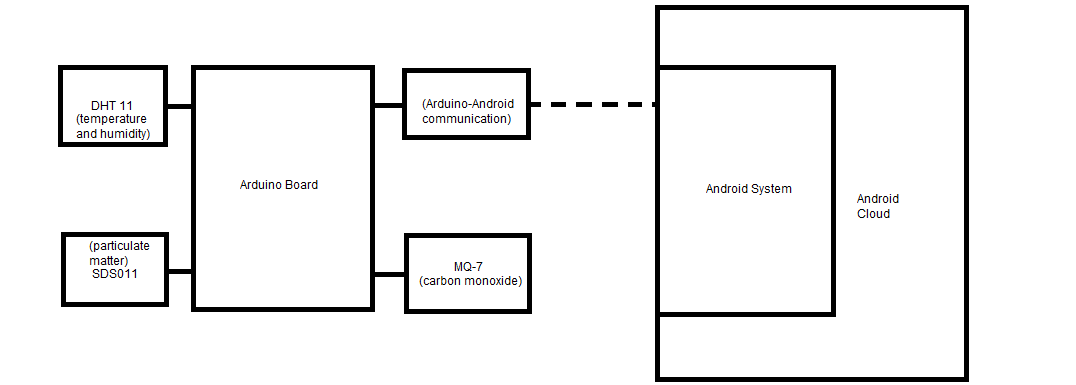
\includegraphics[width=\textwidth]{BlockDiagram}

\begin{center}
Figure 4.1. System Model of the Project
\end{center}

\begin{center}
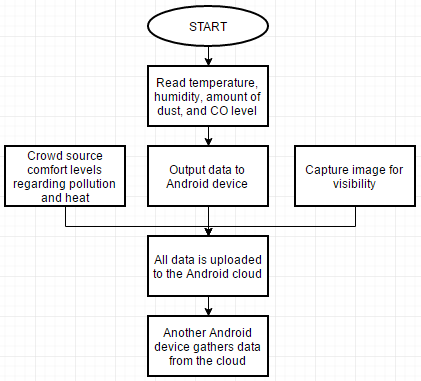
\includegraphics{Flowchart}
\end{center}




\begin{center}
Figure 4.2. System Flowchart
\end{center}

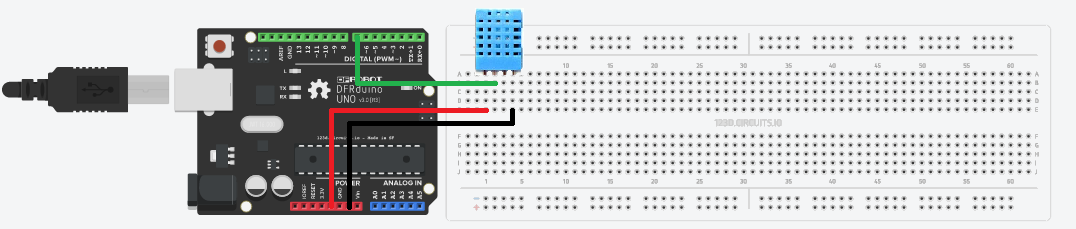
\includegraphics[width=\textwidth]{CurrentProgress}

\begin{center}
Figure 4.3. Circuit Configuration for Testing the DHT-11
\end{center}







\begin{lstlisting}
#include <dht.h>

dht DHT;

#define DHT11_PIN 7

void setup(){
  Serial.begin(9600);
}

void loop()
{
  int chk = DHT.read11(DHT11_PIN);
  Serial.print("Temperature = ");
  Serial.println(DHT.temperature);
  Serial.print("Humidity = ");
  Serial.println(DHT.humidity);
  delay(1000);
}
\end{lstlisting}

\begin{center}
Figure 4.4. Code for Temperature and Humidity Gathering
\end{center}
\begin{center}
\begin{eqnarray}
DI = T-0.55(1-0.01H)(T-14.5)
\label{Discomfort Index}
\end{eqnarray}
\end{center}
\begin{center}
Figure 4.5. Formula for Discomfort Index
\end{center}

\section{Summary}

According to the system model, the project will make use of an Arduino microcontroller system that will handle tasks of gathering inputs which are the temperature, humidity, amount of dust, and amount of carbon monoxide. These data will be transmitted an Android system. Afterwards, this data can be submitted  to the Android cloud in real time. Each individual Android system in the cloud can make use of the camera to capture the image of the surroundings in order to get the visibility with the aid of computer vision. A crowdsourcing element is considered to be added in each system where the user can rank the amount of discomfort he feels in terms of the heat and air pollution. This information will be utilized in the cloud.

The current accomplishments for the group is the successful gathering of the temperature and humidity with the use of the Arduino system and the DHT-11 sensor. These values are rounded to the nearest units value.
\stopcontents[chapters]
\cleardoublepage

%%%%%%%%%%%%%%%%%%%%%%%%%%%%%%%%%%%%%%%%%%%%%%%%
\chapter{Methodology} 
\label{ch:method} 
\startcontents[chapters]
\begin{SingleSpace}	
	\Mprintcontents 
\end{SingleSpace}
\section{Implementation}
The group has chosen system prototyping as the primary methodology of the study Fig. ~\ref{fig:SPD} which comes from [Dennis, 2014]. It is effective to use this because Arduino is quick to learn and would be useful in creating prototypes easily. It will also be advantageous to follow this methodology because of the time constraint and weekly updates. This would, however, not be very effective in terms of developing an Android application with a crowdsourcing element and bluetooth communications due to its unfamiliarity to the group. 

\begin{figure}[h]
	\centering
	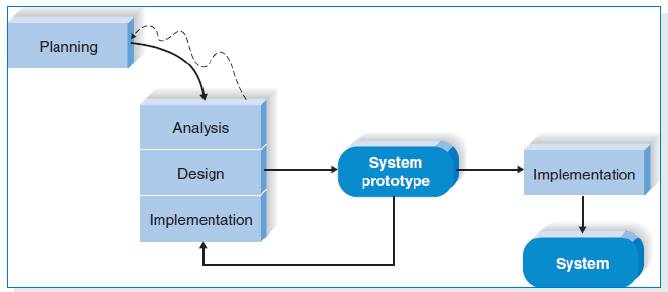
\includegraphics[width=\textwidth]{GraphColor}
	\caption{System Prototyping Diagram}
	\label{fig:SPD}
\end{figure}

\subsection{Planning}
The planning stage took around four weeks. In the planning stage, several factors of air quality was taken into consideration. Among these factors are temperature, humidity, dust, and amount of Carbon Monoxide. In creating this design, few more considerations must be accounted for. Among these are portability, Android compatibility, and real time. Different stages must take place in creating the proposed system. These stages will consist of the integration of the different sensors to our design, testing and evaluating these sensors, and integrating them in the Android application. 

\subsection{Initial Prototype}
For the initial prototype, the temperature and humidity are first taken into consideration. The design will include the DHT11 humidity sensor and an LED display to provide feedback on the current temperature and humidity as well as the discomfort index of the area. Several sets of data are first taken in order to retrieve the temperature and humidity. This is done in order to a check the consistency and accuracy of the measuring devices used for comparing the data collected from our design. The data is taken from 3 different days with 2 analog and 1 digital sensor. The prototype will make use of the DHT11 sensor and and its accuracy will be tested using the best thermometer and hygrometer.

\subsection{Second Prototype}
More features are added in the initial prototype.These will include bluetooth communications with the Android app as well as integrating crowdsourcing using FireBase. This will also include the SDS011 particulate matter laser sensor which measures the concentration of dust present locally. The use of this sensor will have a relative error of 10\% . This error will be tested by comparing the results to a DustTrak or GRIMM dust monitor.

\subsection{Final Prototype} 
Using  MQ-7 CO sensor, the prototype will be further extended. The range will be from 10 to 500 ppm which is sufficient to determine how harmful the amount is. This too will be compared to an existing CO meter which will be used to measure the reliability of the sensor. The final prototype will also include the integration of visibility detection. The visibility detection will make use of OpenCV by making use of Canny Edge Detection. The prototype will also finalize the Android application's features and design.

\subsection{Integration of Communication Devices}
The data transferred will not only be transferred to the proposed Android application but also to a cloud. This will involve crowdsourcing which would enable several data to be inputted at real time. To transfer the data from the proposed system to the Android application, the SMiRF Bluetooth module or HC-05 Bluetooth module will be used. The data collected will then be transferred to a Firebase database. 

\section{Evaluation}

The study is to develop a mobile phone application that utilizes the use of a microcontroller-based system to measure air parameters in getting the discomfort index and amount of air pollutants. The discomfort index is dependent on air parameters measured by the system. In relation to the air parameters, the study uses a quantitative approach of data gathering, through actual measurements of air parameters using analog and digital meters and sensors. A crowdsourcing approach was then applied for better information gathering between the users of the applications across the map. 

\subsection{Quantitative Approach}
Data were gathered four nonconsecutive trials on twenty different locations along De La Salle University. The data collected is consists of the measurements of the available meters, one digital and two analog meters, and the measurements of the actual sensors used on the system. The time and date, when the data were taken, were also recorded due to the fact that the parameters greatly varies on the weather and the time it was measured which also leads to inconsistent recorded data. 

The gathered data were used to determine the reliability of the measurements from the sensors used in the system, in resemblance to the measurements from the meters. The use of the meters are for establishing the ground truth of the measurements of air parameters. Also, the data were ranked according to their corresponding computed level of discomfort or discomfort index based on the parameters measured using both the meters and the sensors.

\subsection{Crowdsourcing Approach}
Due to the fact that the data can only be collected when the user is at the specified location, the android application used in this study integrates a crowdsourcing approach in gathering of data. In this way, the user can be aware of the conditions of the air parameters around a location on the map based on the data from the other users that are in the location. 

The application is capable of sharing or storing information in a cloud for crowdsourcing. The cloud is used to hold the data from all the information stored by each users of the application. The crowdsourcing application is very dependent on the users data and it would be most effective when more people uses the application. This approach allows the user to gather information and at the same time, contributes to the cloud-based system of the application which also contributes to the data gathering of other users.

\section{Summary}
The proposed design will contain several sensors that will measure temperature, humidity, particulate matter amount, and levels of carbon dioxide. There are different stages in gathering the various data required. The sensors will be calibrated based from its individual datasheets. The data will be taken in a span of two weeks and at different times throughout the day. The data taken from our design will be compared with commercial sensors that are readily available to test the reliability and consistency of the proposed design. 

The data collected from DHT11 sensor for detecting temperature and humidity will be measured. The design will also use a SDS011 PM laser sensor to record the amount of dust present within its range. The MQ-7 CO sensor will record the concentrations of Carbon Monoxide in its vicinity. The range will be from 10 to 500 ppm which is sufficient to determine how harmful the amount of Carbon Monoxide is. These will be tested with their corresponding meters and its accuracy will be determined. The data collected will be sent to a database in a cloud and transferred to the Android application. The program within the application will handle the discomfort index calculation and will determine level of discomfort.



\stopcontents[chapters]
\cleardoublepage

%%%%%%%%%%%%%%%%%%%%%%%%%%%%%%%%%%%%%%%%%%%%%%%%
\ifResultDiscuss 
	\chapter{Results and Discussion} 
	\label{ch:result_discuss} 
	\startcontents[chapters]
	\begin{SingleSpace}	
		\Mprintcontents 
	\end{SingleSpace}
	The goal of this research is to be able to provide a system that makes use of an Arduino-based measuring device that can pass on data with a Bluetooth module to an Android phone that can be able to relay this data to a firebase database that can be accessed by another Android phone.

In order to be able to verify the temperature-humidity sensor being used, another device will serve as the basis for true data. Measurements coming from the TH-65, a digital temperature and humidity measuring device, will be established as ground truth.

The following graphs show the accuracy testing of the DHT-11 with the TH-65 as the basis for ground truth. The blue data represents the temperature measured by the DHT-11 while the orange represents data coming from the TH-65. Temperature, humidity, and discomfort index are to be considered in this set of data. From the results, it has been shown that in measuring temperature, the DHT-11 sensor shows 98.91\% accuracy and in humidity, the sensor is 89.66\% accurate in terms of measuring humidity and in discomfort index, the sensor is 97.79\% accurate. %The DHT-11 is shown to be 97.79\% accurate regarding the digital thermometer-hygrometer.

\begin{figure}[h]
\centering
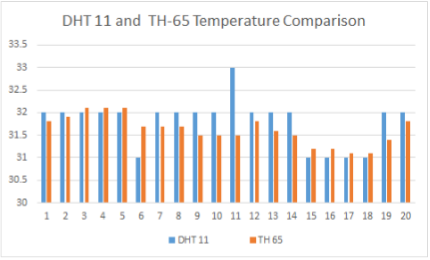
\includegraphics{Temperature}
\caption{Accuracy Testing of Temperature from DHT-11 sensor}
\end{figure}

\begin{figure}[h]
\centering
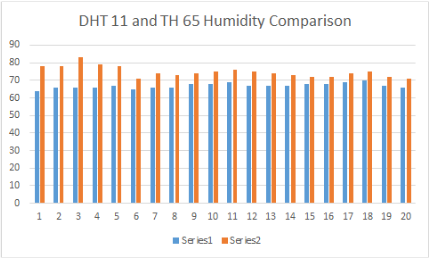
\includegraphics{Humidity}
\caption{Accuracy Testing of Humidity from DHT-11 sensor}
\end{figure}

\begin{figure}[h]
\centering
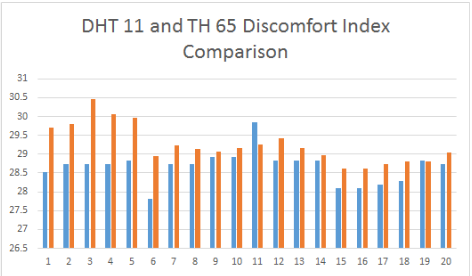
\includegraphics{DI}
\caption{Accuracy Testing of Discomfort Index from DHT-11 sensor}
\end{figure}

The Android application consists of viewing the database, checking the map, and updating the database. In updating the database, the data would simply come from the Arduino system transmitted via Bluetooth. The database is able to view the updated list of temperature, humidity, and discomfort index. The map shows the areas within DLSU that are color coded based on their discomfort indices. If the value shown is less than 21, the marker becomes blue. If it is between 21 to 24, the marker becomes cyan. If it is 24 to 27, the marker becomes azure. If it is between 27 to 29, the marker becomes orange. If it is between 29 to 32, the marker becomes rose. And if it is greater than 32, the marker becomes red.

\begin{figure}[h]
\centering
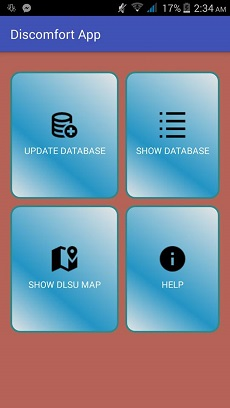
\includegraphics{Interface}
\caption{Interface for the Android Application}
\end{figure}

\begin{figure}[h]
\centering
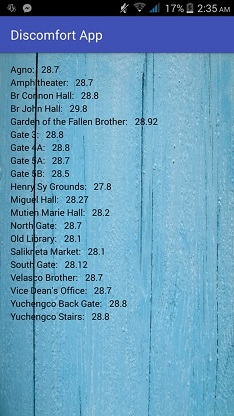
\includegraphics{Firebase}
\caption{The Updated List of Discomfort Indices Viewed from the Map}
\end{figure}

\begin{figure}[h]
\centering
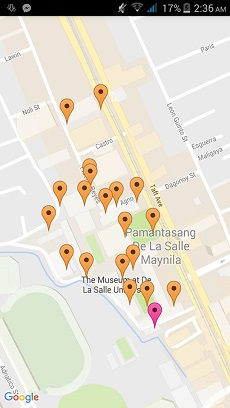
\includegraphics{Map}
\caption{Map of DLSU with Color Coded Markers Dictating the Discomfort Index}
\end{figure}

\begin{figure}[h]
\centering
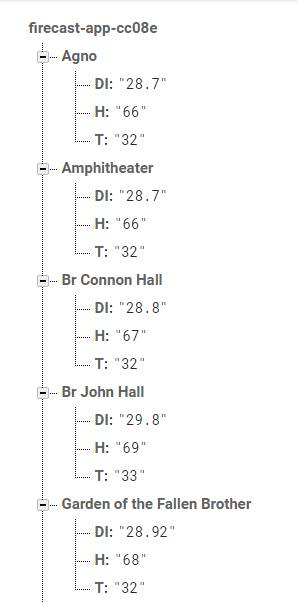
\includegraphics{Database}
\caption{A Part of the Firebase Database}
\end{figure}

\section{Summary}
The group has successfully developed an Arduino-based measuring device that takes note of temperature and humidity which can be transmitted via Bluetooth to an Android device and into an Android application. These data can be relayed onto the firebase database which will be accessible by all who has downloaded the application. The map inside is a handy feature that instantly tells the discomfort level of a certain area inside the university.
	\stopcontents[chapters]
	\cleardoublepage
\fi

%%%%%%%%%%%%%%%%%%%%%%%%%%%%%%%%%%%%%%%%%%%%%%%%
\ifConc
	\chapter{Conclusions, Recommendations, and Future Directives} 
	\label{ch:conc} 
	\startcontents[chapters]
	\begin{SingleSpace}	
		\Mprintcontents 
	\end{SingleSpace}
	\section{Concluding Remarks}

The common function of the Arduino base temperature and humidity meter is to detect the temperature and humidity in any places in order to come up with discomfort index value.  This discomfort computation feature of the Arduino base machine would be a new way of giving information on how students feel inside the university campus.
In this thesis, the group discussed the process and algorithms to detect temperature and humidity and come up with discomfort index value.  The problem that was faced during the development of this research was how to gather the ground truth data and compare it with the data gathered in order to know that it is accurate.  The first method used is analog and digital temperature and humidity meter data gathering.  In comparison, analog and digital humidity and temperature meters showed similar results but digital showed a more accurate data which is nearer to the data gathered in the Arduino temperature and humidity detector machine.  The ground truth was set as data from digital temperature and humidity meter to come up with a more accurate discomfort index result.  On the other hand, the android based application for discomfort index indication used firebase technology for displaying and uploading the humidity, temperature, and discomfort index data.  The data is uploaded in the firebase and displays the data from various locations.  The advantage of this application is that the crowd can easily upload their humidity and temperature data so that everyone application users will know which places are comfortable and which places are not. When this data is transferred into a google map, it will be a heat map of the campus to graphically indicate the discomfort index of different locations.
The project came up with several problems for the temperature and humidity meter machine. There was a challenge that how this machine will get accurate data from the sensor before the ground truth was set as reference. Spreading the informative data to the student was also a problem but the firebase crowd sourcing technology solved the issue. The Android platform application was a better option for the discomfort indicator due to its versatility and expandability, compared to other mobile development platforms.
The hardware presented in this thesis can be further developed into smaller size and come up with more sensors. It can be innovated with the use of dust sensor and carbon monoxide sensors to perform such functionality. This Arduino temperature and humidity meter machine can be of use not only in the campus, but also in any places outside of the university. This application can further touch the area of health awareness and medical information regarding the discomfort index and data gathered.


\section{Contributions}

The interrelated \index{contributions} contributions and supplements that have been developed in this \documentType  are listed as follows.

\begin{itemize}
  \item The construction of an accurate device that measures temperature and humidity
	
	\item The development of an Android application to increase social awareness
  
	
\end{itemize}


\section{Recommendations}

There is more to air pollution than measuring particulate matter and carbon monoxide. It is highly recommended that the measurements of air pollutants be improved by the addition of more sensors to the Arduino system so that more air pollutants and parameters can be measured such as sulfur dioxide and nitrogen dioxide. The system's setting so far is within the campus and the values shown are nearly consistent with one another. It is also recommended to further expand the coverage of taking down the discomfort index in order for more areas to be involved. Since Google Map API was used to take note of the location, another recommended study is to make use of the GPS location to mark that certain area's discomfort levels.

\section{Future Prospects}

There are several prospect related in this research that may be extended for further studies. So the suggested topics are listed in the following.

\begin{enumerate}
	\item  The addition of more air pollutants to be measured.
	
	\item  The expansion of areas that take note of temperature, humidity, and amount of air pollution.
		
\end{enumerate}



	\stopcontents[chapters]
	\cleardoublepage
\fi

%%%%%%%%%%%%%%%%%%%%%%%%%%%%%%%%%%%%%%%%%%%%%%%
\renewcommand{\UrlFont}{\normalfont}
%\bibliographystyle{IEEEtr} % for IEEE referencing format
\bibliographystyle{apalike} % for APA referencing format
\begin{SingleSpace}
	{\small \bibliography{references}}
\end{SingleSpace}
\vfill
\begin{flushright}
Produced: \usdate\today, \currenttime \\
\end{flushright}
\cleardoublepage 

%%%%%%%%%%%%%%%%%%%%%%%%%%%%%%%%%%%%%%%%%%%%%%%%
\SingleSpacing
\appendix
\renewcommand{\thechapter}{\Alph{chapter}}
\renewcommand{\thesection}{\thechapter\arabic{section}}
\appto\appendix{\renewcommand\thechapter{\AlphAlph{\value{chapter}}}} % for increasing appendix chapters beyond Z, i.e. AA, AB, etc.
\chapter{Answers to Questions to this \documentType}
\startcontents[chapters]
\Mprintcontents 



\section{How important is the problem to practice?}

The Philippines is a country that is prone to discomfort due to the inevitable elements of air pollution and rising heat levels. An Android application for awareness can be able to alert the locals about these issues.	
	
\section{How will you know if the solution/s that you will achieve would be better than existing ones?}	

Currently, there are no Android applications that provide real-time updates on discomfort index and amount of dust and carbon monoxide in a Philippine implementation.

\subsection{How will you measure the improvement/s?}	

Improvements could be measured by providing different ground truths (other thermometers/hygrometers) to test the accuracy of the system as well as surveys to confirm the level of discomfort felt by the user. Also, integrating the system to the phone is a way to retrieve data easily and it would occupy less space instead of having two separate systems communicating.
	
\subsubsection{What is/are your basis/bases for the improvement/s?}

The accuracy of the system will be the basis of improvement as well as the apparent level of discomfort felt by the user.
		
\subsubsection{Why did you choose that/those basis/bases?}

These data would not only test the accuracy of the Arduino system but also validate the data with the user's perceived level of discomfort.
				
\subsubsection{How significant are your measure/s of the improvement/s?}

They are significant because the measures of improvement will be more expensive than our system and will determine if a low cost system can be viable alternative to the existing systems.


\section{What is the difference of the solution/s from existing ones?}
	
Weather reports provide temperature and humidity in different parts of the world but our solution combines them both into a discomfort index derived from heat which is an essential factor in the levels of comfort of an individual.

\subsection{How is it different from previous and existing ones?}

Weather stations provide measurements pertaining to temperature and humidity but in this solution, the measurements can be accurately measured with an Arduino-based system. The crowd sourcing element in the research enables these data to be updated time and time again, faster than an selecting an interval of a daily update.

	
\section{What are the assumptions made (that are behind for your proposed solution to work)?}
	
For this research, it is assumed that almost every person in the community owns an Android phone because with this phone, one can access the information from the firebase database.
		
	
\subsection{Will your proposed solution/s be sensitive to these assumptions?}
	
Yes. The entire system designed so far is made for Android phones that are able to access this firebase database.

  
\subsection{Can your proposed solution/s be applied to more general cases when some of the assumptions are eliminated? If so, how?}

In the case of this study, the proposed solution cannot be applied to more general cases. The main backbone of the thesis is the Android system since it gathers the data from the Arduino system and it enables access to the different discomfort indices within the university.


\section{What is the necessity of your approach/proposed solution/s?}

Our solution aims towards the convenience of anyone that has the
	
\subsection{What will be the limits of applicability of your proposed~solution/s?}

As of now, the whole crowdsourcing system is implemented to provide data such as temperature and humidity for various locations within the university only.
					  
\subsection{What will be the message of the proposed solution to technical people?  How about to non-technical managers and business men?}
			
For the technical people, the message would be that it is possible to create an application that uses crowdsourcing to take note of air pollution and discomfort index by the construction of an Arduino system that can transmit data via Bluetooth to an Android device which can pass on the data to the firebase database accessible by anyone who has the application. For the non-technical managers, we would say that an application that takes note of real-time updates of the amount of discomfort based on heat and air pollution has been developed.



\section{How will you know if your proposed solution/s is/are correct?}

The sensors for temperature, humidity, amount of particulate matter, and carbon monoxide content will be tested based on the accuracy in terms of a ground truth. All group members that own Android phones can be able to verify the data.
			
\subsection{Will your results warrant the level of mathematics used (i.e., will the end justify the means)?}
	    
Yes. A mathematical formula in computing the discomfort index that makes use of temperature and humidity was used.
			

\section{Is/are there an/\_ alternative way/s to get to the same solution/s?}

Other microcontroller systems can be considered as alternatives since they also can be able to retrieve values of temperature and humidity with the sensors and transmit the data via Bluetooth or even another method of data transmission.
	
\subsection{Can you come up with illustrating examples, or even better, counter examples to your proposed solution/s?}

In terms of data gathering, the data would vary based on the time the measurements were taken and weather conditions. There are different stations and air quality devices present today such as Netatmo and CubeSensor however these are very expensive to implement.
	
\subsection{Is there an approximation that can arrive at the essentially the same proposed solution/s more easily?}
	
Integrating the system to the smartphone is a way to retrieve data easily and it would occupy less space instead of having two separate systems communicating.
	
	
\section{If you were the examiner of your proposal, how would you present the proposal in another way?}
	
It seems that it would be better if there would be a live system and app demonstration instead of the usual Powerpoint presentation in order to better understand how the system works.
	
\subsection{What are the weaknesses of your proposal?}

The system implemented within the university would yield nearly the same results from different locations.

\stopcontents[chapters]
\cleardoublepage

%%%%%%%%%%%%%%%%%%%%%%%%%%%%%%%%%%%%%%%%%%%%%%%%
\chapter{Usage Examples} 
\label{ch:usage_examples}
% \startcontents[chapters]
% \Mprintcontents  
The user is expected to have a working knowledge of \LaTeX. A good introduction is in~\cite{Oetiker2014}.  Its latest version can be accessed at \url{http://www.ctan.org/tex-archive/info/lshort}.




\section{Equations}
\label{sec:eqn_not}

The following examples show how to typeset equations in \LaTeX.  This section also shows examples of the use of \verb| \gls{ } | commands in conjunction with the items that are in the \verb| notation.tex | file. \textbf{Please make sure that the entries in} \verb| notation.tex |\textbf{  are those that are referenced in the \LaTeX \ document files used by this \documentType.  Please comment out unused notations and be careful with the commas and brackets  in} \verb| notation.tex |.

In~\eqref{eq:conv}, the output signal \gls{not:output_sigt} is the result of the convolution of the input signal \gls{not:input_sigt} and the impulse response \gls{not:ir}.

\begin{eqnarray}   
     y\left( t \right) = h\left( t \right) * x\left( t \right)=\int_{-\infty}^{+\infty}h\left( t-\tau \right)x\left( \tau \right) \mathrm{d}\tau
	\label{eq:conv}
\end{eqnarray}

Other example equations are as follows.

\begin{eqnarray}
	\left[ \dfrac{ V_{1} }{ I_{1} } \right] = 
	\begin{bmatrix}
		A & B \\ 
		C & D 
	\end{bmatrix} 
	\left[ \dfrac{ V_{2} }{ I_{2} } \right]
	\label{eq:ABCD}
\end{eqnarray}

\begin{eqnarray}
\dfrac{1}{2} < \left\lfloor \mathrm{mod}\left(\left\lfloor \dfrac{y}{17} \right\rfloor 2^{-17 \lfloor x \rfloor - \mathrm{mod}(\lfloor y\rfloor, 17)},2\right)\right\rfloor,
\end{eqnarray}

\begin{eqnarray}
| \zeta(x)^3 \zeta(x + iy)^4 \zeta(x + 2iy) | = 
\exp\sum_{n,p} \frac{3 + 4 \cos( ny \log p) + \cos (2ny \log p)}{np^{nx}} \ge 1
\end{eqnarray}

\newpage
The verbatim \LaTeX \ code of Sec.~\ref{sec:eqn_not} is in List.~\ref{lst:eqn_gls}.

\begin{lstlisting}[
float=h,
caption=Sample \LaTeX \ code for equations and notations usage, 
label=lst:eqn_gls,
language=TeX,
frame=single]
The following examples show how to typeset equations in \LaTeX. 

In~\eqref{eq:conv}, the output signal \gls{not:output_sigt} is the result of the convolution of the input signal \gls{not:input_sigt} and the impulse response \gls{not:ir}.

\begin{eqnarray}   
     y\left( t \right) = h\left( t \right) * x\left( t \right)=\int_{-\infty}^{+\infty}h\left( t-\tau \right)x\left( \tau \right) \mathrm{d}\tau
	\label{eq:conv}
\end{eqnarray}

Other example equations are as follows.

\begin{eqnarray}
	\left[ \dfrac{ V_{1} }{ I_{1} } \right] = 
	\begin{bmatrix}
		A & B \\ 
		C & D 
	\end{bmatrix} 
	\left[ \dfrac{ V_{2} }{ I_{2} } \right]
	\label{eq:ABCD}
\end{eqnarray}

\begin{eqnarray}
{1\over 2} < \left\lfloor \mathrm{mod}\left(\left\lfloor {y \over 17} \right\rfloor 2^{-17 \lfloor x \rfloor - \mathrm{mod}(\lfloor y\rfloor, 17)},2\right)\right\rfloor,
\end{eqnarray}

\begin{eqnarray}
| \zeta(x)^3\zeta(x+iy)^4\zeta(x+2iy) | = 
\exp\sum_{n,p}\frac{3+4\cos(ny\log p) +\cos (2ny\log p)}{np^{nx}}\ge 1
\end{eqnarray}
\end{lstlisting}
\cleardoublepage







\newpage
\section{Notations}
\label{sec:not}
In order to use the standardized notation, the user is highly suggested to see the ISO~80000-2 standard~\cite{ISO800002}. The following were taken from \verb| isomath-test.tex |.

% A teststring with Latin and Greek letters::
\newcommand{\teststring}{%
% capital Latin letters
% A,B,C,
A,B,
% capital Greek letters
%\Gamma,\Delta,\Theta,\Lambda,\Xi,\Pi,\Sigma,\Upsilon,\Phi,\Psi,
\Gamma,\Delta,\Theta,\Lambda,\Xi,\Pi,\Sigma,\Phi,\Psi,\Omega,
% small Greek letters
\alpha,\beta,\pi,\nu,\omega,
% small Latin letters:
% compare \nu, \omega, v, and w
v,w,
% digits
0,1,9
}


\subsection*{Math alphabets}

If there are other symbols in place of Greek letters in a math
alphabet, it uses T1 or OT1 font encoding instead of OML.

\begin{eqnarray*}
\mbox{mathnormal} &  & \teststring \\
\mbox{mathit} &  & \mathit{\teststring}\\
\mbox{mathrm} &  & \mathrm{\teststring}\\
\mbox{mathbf} &  & \mathbf{\teststring}\\
\mbox{mathsf} &  & \mathsf{\teststring}\\
\mbox{mathtt} &  & \mathtt{\teststring}
\end{eqnarray*}
 New alphabets bold-italic, sans-serif-italic, and sans-serif-bold-italic.
\begin{eqnarray*}
\mbox{mathbfit}     &  & \mathbfit{\teststring}\\
\mbox{mathsfit}     &  & \mathsfit{\teststring}\\
\mbox{mathsfbfit} &  & \mathsfbfit{\teststring}
\end{eqnarray*}
%
Do the math alphabets match?

$
\mathnormal  {a x \alpha \omega}
\mathbfit    {a x \alpha \omega}
\mathsfbfit{a x \alpha \omega}
\quad
\mathsfbfit{T C \Theta \Gamma}
\mathbfit    {T C \Theta \Gamma}
\mathnormal  {T C \Theta \Gamma}
$

\subsection*{Vector symbols}

Alphabetic symbols for vectors are boldface italic,
$\vec{\lambda}=\vec{e}_{1}\cdot\vec{a}$,
while numeric ones (e.g. the zero vector) are bold upright,
$\vec{a} + \vec{0} = \vec{a}$.

\subsection*{Matrix symbols}

Symbols for matrices are boldface italic, too:%
\footnote{However, matrix symbols are usually capital letters whereas vectors
are small ones. Exceptions are physical quantities like the force
vector $\vec{F}$ or the electrical field $\vec{E}$.%
}
$\matrixsym{\Lambda}=\matrixsym{E}\cdot\matrixsym{A}.$


\subsection*{Tensor symbols}

Symbols for tensors are sans-serif bold italic,

\[
   \tensorsym{\alpha}  =  \tensorsym{e}\cdot\tensorsym{a}
   \quad \Longleftrightarrow \quad
   \alpha_{ijl}  =  e_{ijk}\cdot a_{kl}.
\]


The permittivity tensor describes the coupling of electric field and
displacement: \[
\vec{D}=\epsilon_{0}\tensorsym{\epsilon}_{\mathrm{r}}\vec{E}\]



\newpage
\subsection*{Bold math version}

The ``bold'' math version is selected with the commands
\verb+\boldmath+ or \verb+\mathversion{bold}+

{\boldmath
	\begin{eqnarray*}
	\mbox{mathnormal} &  & \teststring \\
	\mbox{mathit} &  & \mathit{\teststring}\\
	\mbox{mathrm} &  & \mathrm{\teststring}\\
	\mbox{mathbf} &  & \mathbf{\teststring}\\
	\mbox{mathsf} &  & \mathsf{\teststring}\\
	\mbox{mathtt} &  & \mathtt{\teststring}
	\end{eqnarray*}
	 New alphabets bold-italic, sans-serif-italic, and sans-serif-bold-italic.
	\begin{eqnarray*}
	\mbox{mathbfit}     &  & \mathbfit{\teststring}\\
	\mbox{mathsfit}     &  & \mathsfit{\teststring}\\
	\mbox{mathsfbfit} &  & \mathsfbfit{\teststring}
	\end{eqnarray*}
	%
	Do the math alphabets match?

	$
	\mathnormal  {a x \alpha \omega}
	\mathbfit    {a x \alpha \omega}
	\mathsfbfit{a x \alpha \omega}
	\quad
	\mathsfbfit{T C \Theta \Gamma}
	\mathbfit    {T C \Theta \Gamma}
	\mathnormal  {T C \Theta \Gamma}
	$

	\subsection*{Vector symbols}

	Alphabetic symbols for vectors are boldface italic,
	$\vec{\lambda}=\vec{e}_{1}\cdot\vec{a}$,
	while numeric ones (e.g. the zero vector) are bold upright,
	$\vec{a} + \vec{0} = \vec{a}$.




	\subsection*{Matrix symbols}

	Symbols for matrices are boldface italic, too:%
	\footnote{However, matrix symbols are usually capital letters whereas vectors
	are small ones. Exceptions are physical quantities like the force
	vector $\vec{F}$ or the electrical field $\vec{E}$.%
	}
	$\matrixsym{\Lambda}=\matrixsym{E}\cdot\matrixsym{A}.$


	\subsection*{Tensor symbols}

	Symbols for tensors are sans-serif bold italic,

	\[
		 \tensorsym{\alpha}  =  \tensorsym{e}\cdot\tensorsym{a}
		 \quad \Longleftrightarrow \quad
		 \alpha_{ijl}  =  e_{ijk}\cdot a_{kl}.
	\]

	The permittivity tensor describes the coupling of electric field and
	displacement: \[
	\vec{D}=\epsilon_{0}\tensorsym{\epsilon}_{\mathrm{r}}\vec{E}\]
}











\newpage
The verbatim \LaTeX \ code of Sec.~\ref{sec:not} is in List.~\ref{lst:not}.

\begin{lstlisting}[
%float=h,% do not use float option for long listings
caption=Sample \LaTeX \ code for notations usage, 
label=lst:not,
language=TeX,
frame=single]
% A teststring with Latin and Greek letters::
\newcommand{\teststring}{%
% capital Latin letters
% A,B,C,
A,B,
% capital Greek letters
%\Gamma,\Delta,\Theta,\Lambda,\Xi,\Pi,\Sigma,\Upsilon,\Phi,\Psi,
\Gamma,\Delta,\Theta,\Lambda,\Xi,\Pi,\Sigma,\Phi,\Psi,\Omega,
% small Greek letters
\alpha,\beta,\pi,\nu,\omega,
% small Latin letters:
% compare \nu, \omega, v, and w
v,w,
% digits
0,1,9
}


\subsection*{Math alphabets}

If there are other symbols in place of Greek letters in a math
alphabet, it uses T1 or OT1 font encoding instead of OML.

\begin{eqnarray*}
\mbox{mathnormal} &  & \teststring \\
\mbox{mathit} &  & \mathit{\teststring}\\
\mbox{mathrm} &  & \mathrm{\teststring}\\
\mbox{mathbf} &  & \mathbf{\teststring}\\
\mbox{mathsf} &  & \mathsf{\teststring}\\
\mbox{mathtt} &  & \mathtt{\teststring}
\end{eqnarray*}
 New alphabets bold-italic, sans-serif-italic, and sans-serif-bold-italic.
\begin{eqnarray*}
\mbox{mathbfit}     &  & \mathbfit{\teststring}\\
\mbox{mathsfit}     &  & \mathsfit{\teststring}\\
\mbox{mathsfbfit} &  & \mathsfbfit{\teststring}
\end{eqnarray*}
%
Do the math alphabets match?

$
\mathnormal  {a x \alpha \omega}
\mathbfit    {a x \alpha \omega}
\mathsfbfit{a x \alpha \omega}
\quad
\mathsfbfit{T C \Theta \Gamma}
\mathbfit    {T C \Theta \Gamma}
\mathnormal  {T C \Theta \Gamma}
$

\subsection*{Vector symbols}

Alphabetic symbols for vectors are boldface italic,
$\vec{\lambda}=\vec{e}_{1}\cdot\vec{a}$,
while numeric ones (e.g. the zero vector) are bold upright,
$\vec{a} + \vec{0} = \vec{a}$.

\subsection*{Matrix symbols}

Symbols for matrices are boldface italic, too:%
\footnote{However, matrix symbols are usually capital letters whereas vectors
are small ones. Exceptions are physical quantities like the force
vector $\vec{F}$ or the electrical field $\vec{E}$.%
}
$\matrixsym{\Lambda}=\matrixsym{E}\cdot\matrixsym{A}.$


\subsection*{Tensor symbols}

Symbols for tensors are sans-serif bold italic,

\[
   \tensorsym{\alpha}  =  \tensorsym{e}\cdot\tensorsym{a}
   \quad \Longleftrightarrow \quad
   \alpha_{ijl}  =  e_{ijk}\cdot a_{kl}.
\]


The permittivity tensor describes the coupling of electric field and
displacement: \[
\vec{D}=\epsilon_{0}\tensorsym{\epsilon}_{\mathrm{r}}\vec{E}\]



\newpage
\subsection*{Bold math version}

The ``bold'' math version is selected with the commands
\verb+\boldmath+ or \verb+\mathversion{bold}+

{\boldmath
	\begin{eqnarray*}
	\mbox{mathnormal} &  & \teststring \\
	\mbox{mathit} &  & \mathit{\teststring}\\
	\mbox{mathrm} &  & \mathrm{\teststring}\\
	\mbox{mathbf} &  & \mathbf{\teststring}\\
	\mbox{mathsf} &  & \mathsf{\teststring}\\
	\mbox{mathtt} &  & \mathtt{\teststring}
	\end{eqnarray*}
	 New alphabets bold-italic, sans-serif-italic, and sans-serif-bold-italic.
	\begin{eqnarray*}
	\mbox{mathbfit}     &  & \mathbfit{\teststring}\\
	\mbox{mathsfit}     &  & \mathsfit{\teststring}\\
	\mbox{mathsfbfit} &  & \mathsfbfit{\teststring}
	\end{eqnarray*}
	%
	Do the math alphabets match?

	$
	\mathnormal  {a x \alpha \omega}
	\mathbfit    {a x \alpha \omega}
	\mathsfbfit{a x \alpha \omega}
	\quad
	\mathsfbfit{T C \Theta \Gamma}
	\mathbfit    {T C \Theta \Gamma}
	\mathnormal  {T C \Theta \Gamma}
	$

	\subsection*{Vector symbols}

	Alphabetic symbols for vectors are boldface italic,
	$\vec{\lambda}=\vec{e}_{1}\cdot\vec{a}$,
	while numeric ones (e.g. the zero vector) are bold upright,
	$\vec{a} + \vec{0} = \vec{a}$.




	\subsection*{Matrix symbols}

	Symbols for matrices are boldface italic, too:%
	\footnote{However, matrix symbols are usually capital letters whereas vectors
	are small ones. Exceptions are physical quantities like the force
	vector $\vec{F}$ or the electrical field $\vec{E}$.%
	}
	$\matrixsym{\Lambda}=\matrixsym{E}\cdot\matrixsym{A}.$


	\subsection*{Tensor symbols}

	Symbols for tensors are sans-serif bold italic,

	\[
		 \tensorsym{\alpha}  =  \tensorsym{e}\cdot\tensorsym{a}
		 \quad \Longleftrightarrow \quad
		 \alpha_{ijl}  =  e_{ijk}\cdot a_{kl}.
	\]

	The permittivity tensor describes the coupling of electric field and
	displacement: \[
	\vec{D}=\epsilon_{0}\tensorsym{\epsilon}_{\mathrm{r}}\vec{E}\]
}

\end{lstlisting}
\cleardoublepage











\newpage
\section{Abbreviation}\
\label{sec:abbrv}

This section shows examples of the use of \LaTeX commands in conjunction with the items that are in the \verb| abbreviation.tex | and in the \verb| glossary.tex | files.  Please see List.~\ref{lst:abbrv}. \textbf{To lessen the \LaTeX \ compilation time, it is suggested that you use} \verb| \acr{ } | \textbf{only for the first occurrence of the word to be abbreviated.}

Again please see List.~\ref{lst:abbrv}. Here is an example of first use: \acr{ac}. Next use: \acr{ac}. Full: \gls{ac}.  Here's an acronym referenced using \verb| \acr |: \acr{html}.  And here it is again: \acr{html}. If you are used to the \texttt{glossaries} package, note the difference in using \verb| \gls |: \gls{html}. And again (no difference): \gls{html}. Here are some more entries:

\begin{itemize}

	\item \acr{xml} and \acr{css}.

	\item Next use: \acr{xml} and \acr{css}.

	\item Full form: \gls{xml} and \gls{css}.

	\item Reset again. \glsresetall{abbreviation}

	\item Start with a capital. \Acr{html}.

	\item Next: \Acr{html}. Full: \Gls{html}.

	\item Prefer capitals? \renewcommand{\acronymfont}[1]{\MakeTextUppercase{#1}} \Acr{xml}. Next: \acr{xml}. Full: \gls{xml}.

	\item Prefer small-caps? \renewcommand{\acronymfont}[1]{\textsc{#1}} \Acr{css}. Next: \acr{css}. Full: \gls{css}.

	\item Resetting all acronyms.\glsresetall{abbreviation}

	\item Here are the acronyms again:

	\item \Acr{html}, \acr{xml} and \acr{css}.

	\item Next use: \Acr{html}, \acr{xml} and \acr{css}.

	\item Full form: \Gls{html}, \gls{xml} and \gls{css}.

	\item Provide your own link text: \glslink{[textbf]css}{style sheet}.

\end{itemize}



The verbatim \LaTeX \ code of Sec.~\ref{sec:abbrv} is in List.~\ref{lst:abbrv}.

\begin{lstlisting}[
float=h,
caption=Sample \LaTeX \ code for abbreviations usage, 
label=lst:abbrv,
language=TeX,
frame=single]
Again please see List.~\ref{lst:abbrv}. Here is an example of first use: \acr{ac}. Next use: \acr{ac}. Full: \gls{ac}.  Here's an acronym referenced using \verb| \acr |: \acr{html}.  And here it is again: \acr{html}. If you are used to the \texttt{glossaries} package, note the difference in using \verb| \gls |: \gls{html}. And again (no difference): \gls{html}. Here are some more entries:

\begin{itemize}

	\item \acr{xml} and \acr{css}.

	\item Next use: \acr{xml} and \acr{css}.

	\item Full form: \gls{xml} and \gls{css}.

	\item Reset again. \glsresetall{abbreviation}

	\item Start with a capital. \Acr{html}.

	\item Next: \Acr{html}. Full: \Gls{html}.

	\item Prefer capitals? \renewcommand{\acronymfont}[1]{\MakeTextUppercase{#1}} \Acr{xml}. Next: \acr{xml}. Full: \gls{xml}.

	\item Prefer small-caps? \renewcommand{\acronymfont}[1]{\textsc{#1}} \Acr{css}. Next: \acr{css}. Full: \gls{css}.

	\item Resetting all acronyms.\glsresetall{abbreviation}

	\item Here are the acronyms again:

	\item \Acr{html}, \acr{xml} and \acr{css}.

	\item Next use: \Acr{html}, \acr{xml} and \acr{css}.

	\item Full form: \Gls{html}, \gls{xml} and \gls{css}.

	\item Provide your own link text: \glslink{[textbf]css}{style} 
	
\end{itemize}
\end{lstlisting}
\cleardoublepage






\newpage
\section{Glossary}
\label{sec:glos}

This section shows examples of the use of \verb| \gls{ } | commands in conjunction with the items that are in the \verb| glossary.tex | and \verb| notation.tex | files.  Note that entries in  \verb| notation.tex |  are prefixed with ``\verb| not: |'' label (see List.~\ref{lst:glos}).

\textbf{Please make sure that the entries in} \verb| notation.tex |\textbf{  are those that are referenced in the \LaTeX \ document files used by this \documentType.  Please comment out unused notations and be careful with the commas and brackets  in} \verb| notation.tex |.

\begin{itemize}

	\item \Glspl{matrix} are usually denoted by a bold capital letter, such as $\mathbfit{A}$. The \gls{matrix}'s $(i,j)$th element is usually denoted $a_{ij}$. \Gls{matrix} $\mathbf{I}$ is the identity \gls{matrix}.

	\item A set, denoted as \gls{not:set}, is a collection of objects.

	\item The universal set,  denoted as \gls{not:universalSet}, is the set of everything.

	\item The empty set, denoted as \gls{not:emptySet}, contains no elements.

	\item The cardinality of a set, denoted as \gls{not:cardinality}, is the number of elements in the set.

\end{itemize}


The verbatim \LaTeX \ code for the part of Sec.~\ref{sec:glos} is in List.~\ref{lst:glos}.

\begin{lstlisting}[
float=h,
caption=Sample \LaTeX \ code for glossary and notations usage, 
label=lst:glos,
language=TeX,
frame=single]
\begin{itemize}

	\item \Glspl{matrix} are usually denoted by a bold capital letter, such as $\mathbfit{A}$. The \gls{matrix}'s $(i,j)$th element is usually denoted $a_{ij}$. \Gls{matrix} $\mathbf{I}$ is the identity \gls{matrix}.

	\item A set, denoted as \gls{not:set}, is a collection of objects.

	\item The universal set,  denoted as \gls{not:universalSet}, is the set of everything.

	\item The empty set, denoted as \gls{not:emptySet}, contains no elements.

	\item The cardinality of a set, denoted as \gls{not:cardinality}, is the number of elements in the set.

\end{enumerate}
\end{lstlisting}
\cleardoublepage












\newpage
\section{Figure}

This section shows several ways of placing figures.  PDF\LaTeX \ compatible files are PDF, PNG, and JPG.  Please see the \verb| figure | subdirectory.

\begin{figure}[!htbp]
	\centering
		
\includegraphics[width=0.5\textwidth]{example}
	\caption{A quadrilateral image example.}
	\label{fig:example}
\end{figure}
\cleardoublepage

Fig.~\ref{fig:example} is a gray box enclosed by a dark border. List.~\ref{lst:onefig} shows the corresponding \LaTeX \ code. 


\begin{lstlisting}[
float=h,
caption=Sample \LaTeX \ code for a single figure, 
label=lst:onefig,
language=TeX,
frame=single]
\begin{figure}[!htbp]
	\centering
		
\includegraphics[width=0.5\textwidth]{example}
	\caption{A quadrilateral image example.}
	\label{fig:example}
\end{figure}
\cleardoublepage

Fig.~\ref{fig:example} is a gray box enclosed by a dark border. List.~\ref{lst:onefig} shows the corresponding \LaTeX \ code. 	
\end{figure}
\end{lstlisting}
\cleardoublepage





\begin{figure}[!htbp]
\centering
\subbottom[A sub-figure in the top row.]{

\includegraphics[width=0.35\textwidth]{example}
\label{fig:top}
}
\vfill
\subbottom[A sub-figure in the middle row.]{

\includegraphics[width=0.35\textwidth]{example}
\label{fig:mid}
}
\vfill
\subbottom[A sub-figure in the bottom row.]{

\includegraphics[width=0.35\textwidth]{example}
\label{fig:botm}
}
\caption{Figures on top of each other. See List.~\ref{lst:figsontop} for the corresponding \LaTeX \ code. } 
\label{fig:tmb}
\end{figure}
\cleardoublepage




\begin{lstlisting}[
float=h,
caption=Sample \LaTeX \ code for three figures on top of each other, 
label=lst:figsontop,
language=TeX,
frame=single]
\begin{figure}[!htbp]
\centering
\subbottom[A sub-figure in the top row.]{

\includegraphics[width=0.35\textwidth]{example}
\label{fig:top}
}
\vfill
\subbottom[A sub-figure in the middle row.]{

\includegraphics[width=0.35\textwidth]{example}
\label{fig:mid}
}
\vfill
\subbottom[A sub-figure in the bottom row.]{

\includegraphics[width=0.35\textwidth]{example}
\label{fig:botm}
}
\caption{Figures on top of each other} 
\label{fig:tmb}
\end{figure}
\end{lstlisting}
\cleardoublepage







\begin{figure}[!htbp]
\centering
\subbottom[A sub-figure in the upper-left corner.]{

\includegraphics[width=0.45\textwidth]{example}
\label{fig:upprleft}
}
\hfill
\subbottom[A sub-figure in the upper-right corner.]{

\includegraphics[width=0.45\textwidth]{example}
\label{fig:uppright}
}
\vfill
\subbottom[A sub-figure in the lower-left corner.]{

\includegraphics[width=0.45\textwidth]{example}
\label{fig:lowerleft}
}
\hfill
\subbottom[A sub-figure in the lower-right corner]{

\includegraphics[width=0.45\textwidth]{example}
\label{fig:lowright}
}
\caption{Four figures in each corner. See List.~\ref{lst:fourfigs} for the corresponding \LaTeX \ code.} 
\label{fig:fourfig}
\end{figure}
\cleardoublepage




\begin{lstlisting}[
float=h,
caption=Sample \LaTeX \ code for the four figures, 
label=lst:fourfigs,
language=TeX,
frame=single]
\begin{figure}[!htbp]
\centering
\subbottom[A sub-figure in the upper-left corner.]{

\includegraphics[width=0.45\textwidth]{example}
\label{fig:upprleft}
}
\hfill
\subbottom[A sub-figure in the upper-right corner.]{

\includegraphics[width=0.45\textwidth]{example}
\label{fig:uppright}
}
\vfill
\subbottom[A sub-figure in the lower-left corner.]{

\includegraphics[width=0.45\textwidth]{example}
\label{fig:lowerleft}
}
\hfill
\subbottom[A sub-figure in the lower-right corner]{

\includegraphics[width=0.45\textwidth]{example}
\label{fig:lowright}
}
\caption{Four figures in each corner. See List.~\ref{lst:fourfigs} for the corresponding \LaTeX \ code.} 
\label{fig:fourfig}
\end{figure}
\end{lstlisting}
\cleardoublepage





\newpage
\section{Table}

This section shows an example of placing a table (a long one). Table~\ref{tab:triple_grid} are the triples. 

\begin{center}
{\scriptsize
\begin{tabularx}{\textwidth}{p{0.1\textwidth}|p{0.2\textwidth}|p{0.5\textwidth}}
\caption{Feasible triples for highly variable grid} \label{tab:triple_grid} \\
\hline 
\hline 
\textbf{Time (s)} & 
\textbf{Triple chosen} & 
\textbf{Other feasible triples} \\ 
\hline 
\endfirsthead
\multicolumn{3}{c}%
{\textit{Continued from previous page}} \\
\hline
\hline 
\textbf{Time (s)} & 
\textbf{Triple chosen} & 
\textbf{Other feasible triples} \\ 
\hline 
\endhead
\hline 
\multicolumn{3}{r}{\textit{Continued on next page}} \\ 
\endfoot
\hline 
\endlastfoot
\hline

0 & (1, 11, 13725) & (1, 12, 10980), (1, 13, 8235), (2, 2, 0), (3, 1, 0) \\
2745 & (1, 12, 10980) & (1, 13, 8235), (2, 2, 0), (2, 3, 0), (3, 1, 0) \\
5490 & (1, 12, 13725) & (2, 2, 2745), (2, 3, 0), (3, 1, 0) \\
8235 & (1, 12, 16470) & (1, 13, 13725), (2, 2, 2745), (2, 3, 0), (3, 1, 0) \\
10980 & (1, 12, 16470) & (1, 13, 13725), (2, 2, 2745), (2, 3, 0), (3, 1, 0) \\
13725 & (1, 12, 16470) & (1, 13, 13725), (2, 2, 2745), (2, 3, 0), (3, 1, 0) \\
16470 & (1, 13, 16470) & (2, 2, 2745), (2, 3, 0), (3, 1, 0) \\
19215 & (1, 12, 16470) & (1, 13, 13725), (2, 2, 2745), (2, 3, 0), (3, 1, 0) \\
21960 & (1, 12, 16470) & (1, 13, 13725), (2, 2, 2745), (2, 3, 0), (3, 1, 0) \\
24705 & (1, 12, 16470) & (1, 13, 13725), (2, 2, 2745), (2, 3, 0), (3, 1, 0) \\
27450 & (1, 12, 16470) & (1, 13, 13725), (2, 2, 2745), (2, 3, 0), (3, 1, 0) \\
30195 & (2, 2, 2745) & (2, 3, 0), (3, 1, 0) \\
32940 & (1, 13, 16470) & (2, 2, 2745), (2, 3, 0), (3, 1, 0) \\
35685 & (1, 13, 13725) & (2, 2, 2745), (2, 3, 0), (3, 1, 0) \\
38430 & (1, 13, 10980) & (2, 2, 2745), (2, 3, 0), (3, 1, 0) \\
41175 & (1, 12, 13725) & (1, 13, 10980), (2, 2, 2745), (2, 3, 0), (3, 1, 0) \\
43920 & (1, 13, 10980) & (2, 2, 2745), (2, 3, 0), (3, 1, 0) \\
46665 & (2, 2, 2745) & (2, 3, 0), (3, 1, 0) \\
49410 & (2, 2, 2745) & (2, 3, 0), (3, 1, 0) \\
52155 & (1, 12, 16470) & (1, 13, 13725), (2, 2, 2745), (2, 3, 0), (3, 1, 0) \\
54900 & (1, 13, 13725) & (2, 2, 2745), (2, 3, 0), (3, 1, 0) \\
57645 & (1, 13, 13725) & (2, 2, 2745), (2, 3, 0), (3, 1, 0) \\
60390 & (1, 12, 13725) & (2, 2, 2745), (2, 3, 0), (3, 1, 0) \\
63135 & (1, 13, 16470) & (2, 2, 2745), (2, 3, 0), (3, 1, 0) \\
65880 & (1, 13, 16470) & (2, 2, 2745), (2, 3, 0), (3, 1, 0) \\
68625 & (2, 2, 2745) & (2, 3, 0), (3, 1, 0) \\
71370 & (1, 13, 13725) & (2, 2, 2745), (2, 3, 0), (3, 1, 0) \\
74115 & (1, 12, 13725) & (2, 2, 2745), (2, 3, 0), (3, 1, 0) \\
76860 & (1, 13, 13725) & (2, 2, 2745), (2, 3, 0), (3, 1, 0) \\
79605 & (1, 13, 13725) & (2, 2, 2745), (2, 3, 0), (3, 1, 0) \\
82350 & (1, 12, 13725) & (2, 2, 2745), (2, 3, 0), (3, 1, 0) \\
85095 & (1, 12, 13725) & (1, 13, 10980), (2, 2, 2745), (2, 3, 0), (3, 1, 0) \\
87840 & (1, 13, 16470) & (2, 2, 2745), (2, 3, 0), (3, 1, 0) \\
90585 & (1, 13, 16470) & (2, 2, 2745), (2, 3, 0), (3, 1, 0) \\
93330 & (1, 13, 13725) & (2, 2, 2745), (2, 3, 0), (3, 1, 0) \\
96075 & (1, 13, 16470) & (2, 2, 2745), (2, 3, 0), (3, 1, 0) \\
98820 & (1, 13, 16470) & (2, 2, 2745), (2, 3, 0), (3, 1, 0) \\
101565 & (1, 13, 13725) & (2, 2, 2745), (2, 3, 0), (3, 1, 0) \\
104310 & (1, 13, 16470) & (2, 2, 2745), (2, 3, 0), (3, 1, 0) \\
107055 & (1, 13, 13725) & (2, 2, 2745), (2, 3, 0), (3, 1, 0) \\
109800 & (1, 13, 13725) & (2, 2, 2745), (2, 3, 0), (3, 1, 0) \\
112545 & (1, 12, 16470) & (1, 13, 13725), (2, 2, 2745), (2, 3, 0), (3, 1, 0) \\
115290 & (1, 13, 16470) & (2, 2, 2745), (2, 3, 0), (3, 1, 0) \\
118035 & (1, 13, 13725) & (2, 2, 2745), (2, 3, 0), (3, 1, 0) \\
120780 & (1, 13, 16470) & (2, 2, 2745), (2, 3, 0), (3, 1, 0) \\
123525 & (1, 13, 13725) & (2, 2, 2745), (2, 3, 0), (3, 1, 0) \\
126270 & (1, 12, 16470) & (1, 13, 13725), (2, 2, 2745), (2, 3, 0), (3, 1, 0) \\
129015 & (2, 2, 2745) & (2, 3, 0), (3, 1, 0) \\
131760 & (2, 2, 2745) & (2, 3, 0), (3, 1, 0) \\
134505 & (1, 13, 16470) & (2, 2, 2745), (2, 3, 0), (3, 1, 0) \\
137250 & (1, 13, 13725) & (2, 2, 2745), (2, 3, 0), (3, 1, 0) \\
139995 & (2, 2, 2745) & (2, 3, 0), (3, 1, 0) \\
142740 & (2, 2, 2745) & (2, 3, 0), (3, 1, 0) \\
145485 & (1, 12, 16470) & (1, 13, 13725), (2, 2, 2745), (2, 3, 0), (3, 1, 0) \\
148230 & (2, 2, 2745) & (2, 3, 0), (3, 1, 0) \\
150975 & (1, 13, 16470) & (2, 2, 2745), (2, 3, 0), (3, 1, 0) \\
153720 & (1, 12, 13725) & (2, 2, 2745), (2, 3, 0), (3, 1, 0) \\
156465 & (1, 13, 13725) & (2, 2, 2745), (2, 3, 0), (3, 1, 0) \\
159210 & (1, 13, 13725) & (2, 2, 2745), (2, 3, 0), (3, 1, 0) \\
161955 & (1, 13, 16470) & (2, 2, 2745), (2, 3, 0), (3, 1, 0) \\
164700 & (1, 13, 13725) & (2, 2, 2745), (2, 3, 0), (3, 1, 0) \\
\end{tabularx}
}
\end{center}
\cleardoublepage









List.~\ref{lst:tabl} shows the corresponding \LaTeX \ code. 

\begin{lstlisting}[
%float=h,% do not use float option for long listings
caption=Sample \LaTeX \ code for making typical table environment, 
label=lst:tabl,
language=TeX,
frame=single,]
\begin{center}
{\scriptsize
\begin{tabularx}{\textwidth}{p{0.1\textwidth}|p{0.2\textwidth}|p{0.5\textwidth}}
\caption{Feasible triples for highly variable grid} \label{tab:triple_grid} \\
\hline 
\hline 
\textbf{Time (s)} & 
\textbf{Triple chosen} & 
\textbf{Other feasible triples} \\ 
\hline 
\endfirsthead
\multicolumn{3}{c}%
{\textit{Continued from previous page}} \\
\hline
\hline 
\textbf{Time (s)} & 
\textbf{Triple chosen} & 
\textbf{Other feasible triples} \\ 
\hline 
\endhead
\hline 
\multicolumn{3}{r}{\textit{Continued on next page}} \\ 
\endfoot
\hline 
\endlastfoot
\hline

0 & (1, 11, 13725) & (1, 12, 10980), (1, 13, 8235), (2, 2, 0), (3, 1, 0) \\
2745 & (1, 12, 10980) & (1, 13, 8235), (2, 2, 0), (2, 3, 0), (3, 1, 0) \\
5490 & (1, 12, 13725) & (2, 2, 2745), (2, 3, 0), (3, 1, 0) \\
8235 & (1, 12, 16470) & (1, 13, 13725), (2, 2, 2745), (2, 3, 0), (3, 1, 0) \\
10980 & (1, 12, 16470) & (1, 13, 13725), (2, 2, 2745), (2, 3, 0), (3, 1, 0) \\
13725 & (1, 12, 16470) & (1, 13, 13725), (2, 2, 2745), (2, 3, 0), (3, 1, 0) \\
16470 & (1, 13, 16470) & (2, 2, 2745), (2, 3, 0), (3, 1, 0) \\
19215 & (1, 12, 16470) & (1, 13, 13725), (2, 2, 2745), (2, 3, 0), (3, 1, 0) \\
21960 & (1, 12, 16470) & (1, 13, 13725), (2, 2, 2745), (2, 3, 0), (3, 1, 0) \\
24705 & (1, 12, 16470) & (1, 13, 13725), (2, 2, 2745), (2, 3, 0), (3, 1, 0) \\
27450 & (1, 12, 16470) & (1, 13, 13725), (2, 2, 2745), (2, 3, 0), (3, 1, 0) \\
30195 & (2, 2, 2745) & (2, 3, 0), (3, 1, 0) \\
32940 & (1, 13, 16470) & (2, 2, 2745), (2, 3, 0), (3, 1, 0) \\
35685 & (1, 13, 13725) & (2, 2, 2745), (2, 3, 0), (3, 1, 0) \\
38430 & (1, 13, 10980) & (2, 2, 2745), (2, 3, 0), (3, 1, 0) \\
41175 & (1, 12, 13725) & (1, 13, 10980), (2, 2, 2745), (2, 3, 0), (3, 1, 0) \\
43920 & (1, 13, 10980) & (2, 2, 2745), (2, 3, 0), (3, 1, 0) \\
46665 & (2, 2, 2745) & (2, 3, 0), (3, 1, 0) \\
49410 & (2, 2, 2745) & (2, 3, 0), (3, 1, 0) \\
52155 & (1, 12, 16470) & (1, 13, 13725), (2, 2, 2745), (2, 3, 0), (3, 1, 0) \\
54900 & (1, 13, 13725) & (2, 2, 2745), (2, 3, 0), (3, 1, 0) \\
57645 & (1, 13, 13725) & (2, 2, 2745), (2, 3, 0), (3, 1, 0) \\
60390 & (1, 12, 13725) & (2, 2, 2745), (2, 3, 0), (3, 1, 0) \\
63135 & (1, 13, 16470) & (2, 2, 2745), (2, 3, 0), (3, 1, 0) \\
65880 & (1, 13, 16470) & (2, 2, 2745), (2, 3, 0), (3, 1, 0) \\
68625 & (2, 2, 2745) & (2, 3, 0), (3, 1, 0) \\
71370 & (1, 13, 13725) & (2, 2, 2745), (2, 3, 0), (3, 1, 0) \\
74115 & (1, 12, 13725) & (2, 2, 2745), (2, 3, 0), (3, 1, 0) \\
76860 & (1, 13, 13725) & (2, 2, 2745), (2, 3, 0), (3, 1, 0) \\
79605 & (1, 13, 13725) & (2, 2, 2745), (2, 3, 0), (3, 1, 0) \\
82350 & (1, 12, 13725) & (2, 2, 2745), (2, 3, 0), (3, 1, 0) \\
85095 & (1, 12, 13725) & (1, 13, 10980), (2, 2, 2745), (2, 3, 0), (3, 1, 0) \\
87840 & (1, 13, 16470) & (2, 2, 2745), (2, 3, 0), (3, 1, 0) \\
90585 & (1, 13, 16470) & (2, 2, 2745), (2, 3, 0), (3, 1, 0) \\
93330 & (1, 13, 13725) & (2, 2, 2745), (2, 3, 0), (3, 1, 0) \\
96075 & (1, 13, 16470) & (2, 2, 2745), (2, 3, 0), (3, 1, 0) \\
98820 & (1, 13, 16470) & (2, 2, 2745), (2, 3, 0), (3, 1, 0) \\
101565 & (1, 13, 13725) & (2, 2, 2745), (2, 3, 0), (3, 1, 0) \\
104310 & (1, 13, 16470) & (2, 2, 2745), (2, 3, 0), (3, 1, 0) \\
107055 & (1, 13, 13725) & (2, 2, 2745), (2, 3, 0), (3, 1, 0) \\
109800 & (1, 13, 13725) & (2, 2, 2745), (2, 3, 0), (3, 1, 0) \\
112545 & (1, 12, 16470) & (1, 13, 13725), (2, 2, 2745), (2, 3, 0), (3, 1, 0) \\
115290 & (1, 13, 16470) & (2, 2, 2745), (2, 3, 0), (3, 1, 0) \\
118035 & (1, 13, 13725) & (2, 2, 2745), (2, 3, 0), (3, 1, 0) \\
120780 & (1, 13, 16470) & (2, 2, 2745), (2, 3, 0), (3, 1, 0) \\
123525 & (1, 13, 13725) & (2, 2, 2745), (2, 3, 0), (3, 1, 0) \\
126270 & (1, 12, 16470) & (1, 13, 13725), (2, 2, 2745), (2, 3, 0), (3, 1, 0) \\
129015 & (2, 2, 2745) & (2, 3, 0), (3, 1, 0) \\
131760 & (2, 2, 2745) & (2, 3, 0), (3, 1, 0) \\
134505 & (1, 13, 16470) & (2, 2, 2745), (2, 3, 0), (3, 1, 0) \\
137250 & (1, 13, 13725) & (2, 2, 2745), (2, 3, 0), (3, 1, 0) \\
139995 & (2, 2, 2745) & (2, 3, 0), (3, 1, 0) \\
142740 & (2, 2, 2745) & (2, 3, 0), (3, 1, 0) \\
145485 & (1, 12, 16470) & (1, 13, 13725), (2, 2, 2745), (2, 3, 0), (3, 1, 0) \\
148230 & (2, 2, 2745) & (2, 3, 0), (3, 1, 0) \\
150975 & (1, 13, 16470) & (2, 2, 2745), (2, 3, 0), (3, 1, 0) \\
153720 & (1, 12, 13725) & (2, 2, 2745), (2, 3, 0), (3, 1, 0) \\
156465 & (1, 13, 13725) & (2, 2, 2745), (2, 3, 0), (3, 1, 0) \\
159210 & (1, 13, 13725) & (2, 2, 2745), (2, 3, 0), (3, 1, 0) \\
161955 & (1, 13, 16470) & (2, 2, 2745), (2, 3, 0), (3, 1, 0) \\
164700 & (1, 13, 13725) & (2, 2, 2745), (2, 3, 0), (3, 1, 0) \\
\end{tabularx}
}
\end{center} 
\end{lstlisting}
\cleardoublepage








\newpage
\section{Algorithm or Pseudocode Listing}

Table~\ref{tab:calcxn} shows an example pseudocode.  Note that if the pseudocode exceeds one page, it can mean that its implementation is not modular.  List.~\ref{lst:algo} shows the corresponding \LaTeX \ code. 

\begin{table}[!htbp]
	\caption{Calculation of $y = x^n$}
	\label{tab:calcxn}
	{\footnotesize
	\begin{tabular}{lll}
	\hline
	\hline
	{\bfseries Input(s):} & & \\
	$n$ & : & $n$th power; $n \in \mathbb{Z}^{+}$ \\
	$x$ & : & base value; $x \in \mathbb{R}^{+}$ \\
	\hline
	{\bfseries Output(s):} & & \\
	$y$ & : & result; $y \in \mathbb{R}^{+}$  \\
	\hline
	\hline
	\\
	\end{tabular}
	}
	\begin{algorithmic}[1]
	{\footnotesize
		\REQUIRE $n \geq 0 \vee x \neq 0$
		\ENSURE $y = x^n$
		\STATE $y \Leftarrow 1$
		\IF{$n < 0$}
				\STATE $X \Leftarrow 1 / x$
				\STATE $N \Leftarrow -n$
		\ELSE
				\STATE $X \Leftarrow x$
				\STATE $N \Leftarrow n$
		\ENDIF
		\WHILE{$N \neq 0$}
				\IF{$N$ is even}
						\STATE $X \Leftarrow X \times X$
						\STATE $N \Leftarrow N / 2$
				\ELSE[$N$ is odd]
						\STATE $y \Leftarrow y \times X$
						\STATE $N \Leftarrow N - 1$
				\ENDIF
		\ENDWHILE
	}	
	\end{algorithmic}
\end{table}
\cleardoublepage




\begin{lstlisting}[
float=h,
caption=Sample \LaTeX \ code for algorithm or pseudocode listing usage, 
label=lst:algo,
language=TeX,
frame=single]
\begin{table}[!htbp]
	\caption{Calculation of $y = x^n$}
	\label{tab:calcxn}
	{\footnotesize
	\begin{tabular}{lll}
	\hline
	\hline
	{\bfseries Input(s):} & & \\
	$n$ & : & $n$th power; $n \in \mathbb{Z}^{+}$ \\
	$x$ & : & base value; $x \in \mathbb{R}^{+}$ \\
	\hline
	{\bfseries Output(s):} & & \\
	$y$ & : & result; $y \in \mathbb{R}^{+}$  \\
	\hline
	\hline
	\\
	\end{tabular}
	}
	\begin{algorithmic}[1]
	{\footnotesize
		\REQUIRE $n \geq 0 \vee x \neq 0$
		\ENSURE $y = x^n$
		\STATE $y \Leftarrow 1$
		\IF{$n < 0$}
				\STATE $X \Leftarrow 1 / x$
				\STATE $N \Leftarrow -n$
		\ELSE
				\STATE $X \Leftarrow x$
				\STATE $N \Leftarrow n$
		\ENDIF
		\WHILE{$N \neq 0$}
				\IF{$N$ is even}
						\STATE $X \Leftarrow X \times X$
						\STATE $N \Leftarrow N / 2$
				\ELSE[$N$ is odd]
						\STATE $y \Leftarrow y \times X$
						\STATE $N \Leftarrow N - 1$
				\ENDIF
		\ENDWHILE
	}	
	\end{algorithmic}
\end{table}
\end{lstlisting}
\cleardoublepage




\newpage
\section{Program/Code Listing}

List.~\ref{lst:fib_c} is a program listing of a C code for computing Fibonacci numbers by calling the actual code. Please see the \verb| code | subdirectory.

\lstinputlisting[
float=h,
caption={[Computing Fibonacci numbers]Computing Fibonacci numbers in C (\lstname) }, 
label=lst:fib_c, 
language=C,
frame=single]{./code/fibo.c}	

List.~\ref{lst:proglist} shows the corresponding \LaTeX \ code. 

\begin{lstlisting}[
float=h,
caption=Sample \LaTeX \ code for program listing, 
label=lst:proglist,
language=TeX,
frame=single]
List.~\ref{lst:fib_c} is a program listing of a C code for computing Fibonacci numbers by calling the actual code. Please see the \verb| code | subdirectory. 
\end{lstlisting}
\cleardoublepage









\newpage
\section{Referencing}
\label{sec:ref}

Referencing chapters: This appendix is in Appendix~\ref{ch:usage_examples}, which is about examples in using various \LaTeX \ commands.

Referencing sections: This section is Sec.~\ref{sec:ref}, which shows how to refer to the locations of various labels that have been placed in the \LaTeX \ files. List.~\ref{lst:refsec} shows the corresponding \LaTeX \ code. 

\begin{lstlisting}[
float=h,
caption=Sample \LaTeX \ code for referencing sections, 
label=lst:refsec,
language=TeX,
frame=single]
Referencing sections: This section is Sec.~\ref{sec:ref}, which shows how to refer to the locations of various labels that have been placed in the \LaTeX \ files. List.~\ref{lst:refsec} shows the corresponding \LaTeX \ code.  
\end{lstlisting}
\blindtext
\cleardoublepage






\subsection{A subsection}
\label{sec:subsec}

Referencing subsections: This section is Sec.~\ref{sec:subsec}, which shows how to refer to a subsection. List.~\ref{lst:refsub} shows the corresponding \LaTeX \ code. 

\begin{lstlisting}[
float=h,
caption=Sample \LaTeX \ code for referencing subsections, 
label=lst:refsub,
language=TeX,
frame=single]
Referencing subsections: This section is Sec.~\ref{sec:subsec}, which shows how to refer to a subsection. List.~\ref{lst:refsub} shows the corresponding \LaTeX \ code. 
\end{lstlisting} 
\blindtext
\cleardoublepage





\subsubsection{A sub-subsection}
\label{sec:subsubsec}


Referencing sub-subsections: This section is Sec.~\ref{sec:subsubsec}, which shows how to refer to a sub-subsection.  List.~\ref{lst:refsubsub} shows the corresponding \LaTeX \ code. 

\begin{lstlisting}[
float=h,
caption=Sample \LaTeX \ code for referencing sub-subsections, 
label=lst:refsubsub,
language=TeX,
frame=single]
Referencing sub-subsections: This section is Sec.~\ref{sec:subsubsec}, which shows how to refer to a sub-subsection. List.~\ref{lst:refsubsub} shows the corresponding \LaTeX \ code. 
\end{lstlisting}

\blindtext
\cleardoublepage







\newpage
\section{Index}

For key words or topics that are expected (or the user would like) to appear in the Index, use \verb| index{key} |, where  \verb| key | is an example keyword to appear in the Index. For example, Fredholm integral and Fourier operator of the following paragraph are in the Index. 

If we make a very large matrix with complex exponentials in the rows (i.e., cosine real parts and sine imaginary parts), and increase the resolution without bound, we approach the kernel of the \index{Fredholm integral} Fredholm integral equation of the 2nd kind, namely the \index{Fourier operator} Fourier operator that defines the continuous Fourier transform. 

List.~\ref{lst:indxsample} is a program listing of the above-mentioned paragraph.

\begin{lstlisting}[
float=h,
caption=Sample \LaTeX \ code for Index usage, 
label=lst:indxsample,
language=TeX,
frame=single]
If we make a very large matrix with complex exponentials in the rows (i.e., cosine real parts and sine imaginary parts), and increase the resolution without bound, we approach the kernel of the \index{Fredholm integral} Fredholm integral equation of the 2nd kind, namely the \index{Fourier} Fourier operator that defines the continuous Fourier transform.
\end{lstlisting}
\cleardoublepage




\newpage
\section{Adding Relevant PDF Pages (e.g. Standards, Datasheets, Specification Sheets, Application Notes, etc.)}

Selected PDF pages can be added (see List.~\ref{lst:pdfpages}), but note that the options must be tweaked.  See the manual of \verb| pdfpages | for other options. 

\begin{lstlisting}[
float=h,
caption=Sample \LaTeX \ code for including PDF pages, 
label=lst:pdfpages,
language=TeX,
frame=single]
\includepdf[pages={8-10},%
offset=3.5mm -10mm,%
scale=0.73,%
frame]
{./reference/Xilinx2015-UltraScaleArchitectureOverview.pdf}
\end{lstlisting}
\cleardoublepage

\includepdf[pages={8-10},%
offset=3.5mm -10mm,%
scale=0.73,%
frame]
{./reference/Xilinx2015-UltraScaleArchitectureOverview.pdf}




	

% \stopcontents[chapters]
\cleardoublepage

%%%%%%%%%%%%%%%%%%%%%%%%%%%%%%%%%%%%%%%%%%%%%%%%
\ifPubList
	\chapter{Publication List and Award}

\flushleft{\Large \bfseries Journal\\}

\begin{enumerate}
\item \ldots

\item \ldots

\end{enumerate}
\vspace{2ex}


\flushleft{\Large \bfseries Conference\\}

\begin{enumerate}

\item \ldots

\item \ldots

\end{enumerate}
\vspace{2ex}



  

\newpage

\flushleft{\Large \bfseries Others}\\
\begin{enumerate}

\item \ldots

\item \ldots

\end{enumerate}
\vspace{2ex}



\flushleft{\Large \bfseries Award}\\

\begin{enumerate}
\item \ldots

\item \ldots
\end{enumerate}
\fi
\cleardoublepage

%%%%%%%%%%%%%%%%%%%%%%%%%%%%%%%%%%%%%%%%%%%%%%%%
\ifVita
	\chapter{Vita}

% Change the descriptions accordingly
%\vfill


\includegraphics[width=0.2\columnwidth]{vita_photo}
\documentAuthor{firstname1} \ \documentAuthor{surname1} \ is a sixth year student at De La Salle University. He is currently taking up his B.Sc. \degree \ studies. His strengths in the field are electronics circuit design and configuration. His fields of interest are electronics hardware and computer microprocessor.


\includegraphics[width=0.2\columnwidth]{vita_photo}
\documentAuthor{firstname2} \ \documentAuthor{surname2} \ is a third year student at De La Salle University. He is currently taking up his B.Sc. \degree \ studies. He has designed communcation systems which covers basic AM radios. His fields of interest are digital communications and computer networks.


\includegraphics[width=0.2\columnwidth]{vita_photo}
\documentAuthor{firstname3} \ \documentAuthor{surname3} \ is a third year student at De La Salle University. He is currently taking up his B.Sc. \degree \ studies.  His strengths in the field are microcontroller program design and advanced electronics.


\includegraphics[width=0.2\columnwidth]{vita_photo}
\documentAuthor{firstname4} \ \documentAuthor{surname4} \ is a fourth year student at De La Salle University. He is currently taking up his B.Sc. \degree \ studies.  He has designed and programmed electronic circuits that includes microcontrollers. His strengths in the field are microcontroller simulation and programming.

%\vfill

\fi
\cleardoublepage

%%%%%%%%%%%%%%%%%%%%%%%%%%%%%%%%%%%%%%%%%%%%%%%%
\ifIndex
	\printindex
\fi
\cleardoublepage

\end{document}